% ==============================================================================
%  $RCSfile: handbuch.tex,v $, $Revision: 1.16 $
%  $Date: 2003/09/20 15:20:25 $
%  $Author: birdy $
%
%  Description: Master Datei des Handbuchs
%
%  Last-Ispelled-Revision:
%
% ==============================================================================

\documentclass[a4paper,titlepage,11pt,german,twoside]{scrbook}

\clearpage
\makeatletter

%koma uses \chapter*, but we want to use \chapter
%  changed srcbook.cls-commands
\renewcommand\idx@heading{%
  \twocolumn
  \chapter{\indexname}\@mkboth{\indexname}{\indexname}
}

%Nummerierung soll net so eng aneinanderhaengen
\renewcommand*\l@section{\@dottedtocline{1}{1.5em}{3em}}

\makeatother


\usepackage{../styles/common}

\usepackage{verbatim}
\usepackage{shortvrb}

\usepackage{handbuch}

\usepackage{makeidx}
\makeindex

% subsubsections nummerieren
\setcounter{secnumdepth}{3}

\newcommand\version{Version 1.2\xspace}
%\newcommand\version{\today\xspace}

% header
\fancyhead{}
\fancyhead[LE,RO]{\slshape \company}
\fancyhead[LO,RE]{\slshape \leftmark}
\fancyfoot[LE,RO]{\thepage{}}
\fancyfoot[LO,RE]{\version}

\begin{document}

% title page
\thispagestyle{empty}
\hfill
\parbox{5.5cm}
{Universit�t Stuttgart\\
Studienprojekt A -- IML Browser\\
\company}

\vspace{3cm}

\begin{center}
  \Huge
  \textsf{Handbuch}\\
  \vspace{.5cm}
  {\Large\version}\\
  \vspace{3cm}
  
\includegraphics[scale=.5]{../logo}
\end{center}
\newpage

\MakeShortVerb{\�}

\section*{Versionsgeschichte}

\begin{itemize}

\item Version 1.0 (08.04.2003)

  Diese Version wurde dem Kunden zur Pr�fung 
  im Kundenreview (14.04.2003 - 16.04.2003) vorgelegt.


\item Version 1.1 (22.04.2003)

  Die Korrekturen gem�� dem Kundenreview vom 14.04.2003 bis
  zum 16.04.2003 wurden eingearbeitet.\\
  Die Spezifikation der GSL (in Version 1.0 noch GQSL) wurde in 
  ein separates Dokument ausgelagert (siehe Kapitel 
  \ref {GIANT Scripting Language}).\\
  Diese Version der Spezifikation ging am 22.04.2003 
  zur Abnahme an den Kunden.

\end{itemize}

%%% Local Variables: 
%%% TeX-master: "spec"
%%% End: 


%===============================================================================
%
% Inhaltsverzeichnis
%
\newpage
\setcounter{tocdepth}{1}
\tableofcontents

%===============================================================================
%
% Einleitung
%
\chapter{Einleitung}
% ==============================================================================
%  $RCSfile: intro.tex,v $, $Revision: 1.2 $
%  $Date: 2003/07/06 13:39:08 $
%  $Author: birdy $
%
%  Description:
%
%  Last-Ispelled-Revision:
%
% ==============================================================================


\section{�ber dieses Dokument}

Dieses Handbuch beschreibt die Installation und Benutzung des graphischen
IML-Browsers GIANT (Graphical IML Analysis Navigation Tool).

\section{�ber GIANT -- Graphical IML Analysis Navigation Tool}
\index{GIANT}
\index{IML-Browser}

GIANT ist ein Werkzeug, welches an der Universit�t Stuttgart von der 
CodeFabrik@Stuttgart im Rahmen des Studienprojektes A IML-Browser 
des Studiengangs Softwaretechnik entwickelt wurde.\\
Ziel dieser Entwicklung war es, die bereits bestehende HTML-basierte L�sung 
der Bauhaus Reengineering GmbH \index{Bauhaus-Reengineering GmbH}
f�r IML-Graphen durch ein komfortables graphisches Werkzeug zu erg�nzen. 
GIANT erm�glicht es dem Kunden, Teile von gro�en IML-Graphen zu
visualisieren. 
Durch die Unterscheidung der verschiedenen Kanten- und Knotenklassen werden
dar�ber hinaus auch im IML-Graphen enthaltene Analyseergebnisse �bersichtlich
dargestellt.\\

\section{Aufbau dieses Dokuments}

In den ersten Kapiteln dieses Handbuches wird beschrieben, wie Anwender
mit GIANT anhand einiger Beispiele Analysen durchf�hren k�nnen.
Dies wird anhand einer Art Tutorials beschrieben. Dies erm�glicht
erfahrenen Anwendern einen schnellen Start (\gq{Top-Down}) mit GIANT.

In den sp�teren Kapiteln wird GIANT Fenster f�r Fenster und Men�punkt
f�r Men�punkt genau erkl�rt (\gq{Bottom-Up}). Dies erm�glicht auch das
Nachschlagen von Details zu einzelnen Funktionen.



%===============================================================================
%
% Produkt�bersicht
%
\chapter{Produkt�bersicht}

In diesem Kapitel werden einige grundlegende Konzepte und
M�glichkeiten von GIANT vorgestellt und kurz beschrieben.

% ==============================================================================
%  $RCSfile: product.tex,v $, $Revision: 1.34 $
%  $Date: 2003/03/31 22:02:25 $
%  $Author: squig $
%
%  Description: Beschreibung des Produktes. �bersicht �ber die Funktionen
%               und allgemeine Bedienkonzepte.
%
%  Last-Ispelled-Revision: 1.32
%
% ==============================================================================


% ==============================================================================
\section{GIANT Projekte} \index{Projekte} \index{Persistenz}

Innerhalb eines Projektes fasst GIANT Informationen, 
wie erzeugte Anzeigefenster und
erzeugte IML-Teilgraphen f�r einen vorgegebenen IML-Graphen, zusammen
und speichert diese persistent. Die Zusammenfassung zu Projekten soll der 
�bersicht dienen und den Austausch von Teilergebnissen, 
wie z.B. einzelner Anzeigefenster, erleichtern.\\
F�r weitere Informationen zu Projekten siehe 
Kapitel \ref{GIANT Projektverwaltung}.


% ==============================================================================
\section{IML-Teilgraphen und Selektionen}
Hinsichtlich der logischen Zusammenfassung von Knoten und Kanten unterscheidet
GIANT IML-Teilgraphen und Selektionen.

  \subsection{IML-Teilgraphen} \index{IML-Teilgraphen}
  \index{Graph-Knoten} \index{Graph-Kanten} \index{hervorheben} Ein
  IML-Teilgraph beschreibt eine Knoten- und Kantenmenge aus dem
  IML-Graphen bei der jede Kante einen Start- und einen Zielknoten hat
  -- die sogenannten Graph-Knoten und Graph-Kanten.  Die Graph-Knoten
  und Graph-Kanten von IML-Teilgraphen k�nnen in Anzeigefenstern
  hervorgehoben werden. Desweiteren k�nnen die Graph-Knoten und
  Graph-Kanten von IML-Teilgraphen als Fenster-Knoten und
  Fenster-Kanten in Anzeigefenster eingef�gt und layoutet werden.  Die
  IML-Teilgraphen sind aber v�llig unabh�ngig von den Anzeigefenstern
  und enthalten insbesondere keine Layoutinformationen.

  \subsection{Selektionen} \index{Selektionen}
  Selektionen stellen die lokale Variante von Knoten- und Kantenmengen dar.
  Sie sind immer einem festen Anzeigefenster zugeordnet.
  Selektionen k�nnen beliebige Knoten und Kanten umfassen, ohne dass diese 
  einen Teilgraphen bilden m�ssen.
  Jeder Knoten und jede Kante einer Selektion muss auch im Anzeigefenster
  als Fenster-Knoten oder Fenster-Kante vorhanden sein.

% ==============================================================================
\section{Anzeigefenster} \index{Anzeigefenster}
Anzeigefenster sind die Fenster von GIANT, in denen eine benutzerdefinierte
Auswahl von Knoten und Kanten visualisiert wird. Es kann beliebig viele
Anzeigefenster geben und jedes Anzeigefenster kann beliebig viele Selektionen
haben.

  \subsection{Pins} \index{Anzeigefenster!Pins} \index{Pins}
  Da bei gro�en Graphen selten alle zu einem Anzeigeinhalt 
  geh�renden Fenster-Knoten und Fenster-Kanten gemeinsam auf dem Bildschirm
  sichtbar dargestellt werden k�nnen, kann sich der
  Benutzer zu jedem Anzeigefenster eine Liste von Pins anlegen. In den Pins wird
  jeweils die Position des sichtbaren Anzeigeinhaltes und die Zoomstufe
  \index{Zoomstufe}
  gespeichert, so dass zu beliebigen Zeitpunkten die Position des sichtbaren
  Anzeigeinhalts rekonstruiert werden kann.

  \subsection{Visualisierungsstile} \index{Visualisierungsstile}
  Mittels sogenannter Visualisierungsstile kann der Benutzer die
  Darstellung von Fenster-Kanten und Fenster-Knoten auch w�hrend der
  Laufzeit von GIANT beeinflussen.  Da �ber entsprechende XML-Dateien
  verschiedene Visualisierungsstile definiert werden k�nnen, kann
  GIANT so
  an spezifische Problemstellungen angepasst werden.\\
  Weitere Informationen hierzu sind unter Abschnitt \ref{Config
    Visualisierungsstile} verf�gbar.

\section{Knoten-Annotationen} \index{Knoten-Annotationen}
Jeder Knoten kann mit einer textuellen Annotation versehen werden. Diese
Annotation kann in einem Fenster au�erhalb des Anzeigefensters
zur Anzeige gebracht und bearbeitet werden.\\
F�r weitere Informationen hierzu siehe Abschnitt
\ref{Project Persistenz von Knoten-Annotationen}.


% ==============================================================================
\section{Anfragen} \index{GQSL} \index{Anfragesprache}
Eine vielseitige Anfragesprache -- die GIANT Query and Scripting Language GQSL --
stellt nahezu die gesamte Funktionalit�t von GIANT zur Verf�gung und kann 
insbesondere auch zum Aufruf via Kommandozeile
genutzt werden. Die drei Schritte des anschlie�end beschriebenen 
\gq{Drei-Stufen-Konzeptes} k�nnen �ber diese Anfragesprache auch \gq{auf 
einen Schlag} erledigt werden.\\
Die GQSL ist unter Kapitel \ref {GIANT Query Skripting Language} im
Detail spezifiziert.


% ==============================================================================
\section{Drei-Stufen-Konzept} \index{Drei-Stufen-Konzept}

Die im Folgenden beschriebenen drei Schritte sollen dem Benutzer die M�glichkeit
bieten, von den Knoten und Kanten des IML-Graphen ausgehend geeignete
Teilgraphen in Anzeigefenstern zu visualisieren. Von der
Gestaltung der UseCases her, werden diese drei Schritte sequentiell nacheinander
ausgef�hrt, dies ist aber nicht zwingend n�tig.


\begin {enumerate}
  \item Erzeugen geeigneter IML-Teilgraphen, d.h.\ Auswahl geeigneter Knoten 
        und Kanten aus dem IML-Graphen mittels der Anfragesprache.
  
  \item Einf�gen dieser IML-Teilgraphen in ein Anzeigefenster unter Anwendung
  eines Layoutalgorithmus \index{Layoutalgorithmen}. 
  
  \item Weitere Bearbeitung der Fenster-Knoten und Fenster-Kanten (wie z.B.
  Verschieben, Annotieren und Erzeugen von Selektionen).
  
\end {enumerate}








%===============================================================================
% 
% Technische Produktumgebung
%
\chapter{Technische Produktumgebung}

Hier wird die zum Betrieb von GIANT n�tige Hardware 
und die n�tige Software sowie die Installation von GIANT
auf Linux-Systemen beschrieben.

% ==============================================================================
%  $RCSfile: technical.tex,v $, $Revision: 1.6 $
%  $Date: 2003/09/23 19:33:38 $
%  $Author: birdy $
%
%  Description: Hier sind die Anforderungen an die Programmumgebung 
%  spezifiziert. Dazu geh�ren die verwendete Hard- und Software, sowie
%  Schnittstellen zu anderen Produkten.
%
%  Last-Ispelled-Revision:
%
% ==============================================================================

\section{Software}

\index{Anforderungen!an die Software}

Zum Betrieb von GIANT wird folgende Hardware und Software ben�tigt:
\begin{itemize}
  \item Sun Solaris, Linux oder Windows Betriebssystem
  \item Emacs oder vi Texteditor f�r die Anzeige vom Sourcecode
  \item GTK 2.0 oder h�her
  \item GTKAda 2.2
\end{itemize}


\section{Hardware}

\index{Anforderungen!an die Hardware}
Das Programm l�uft auf SPARC Workstations und x86 kompatiblen PCs.
Im Folgenden sind die minimalen Hardwareanforderungen zur Arbeit mit kleinen 
und mittleren Projekten beschrieben. 
Bei gro�en Projekten ist ein Speicherausbau
von 2 GB und mehr empfehlenswert.

\subsection{Hardwareanforderungen SPARC}

\begin{itemize}
  \item UltraSPARC-II 300 MHz
  \item 512 MB Hauptspeicher
  \item 8 Bit Grafik mit einer min. Aufl�sung von 1024*786
  \item Maus mit mindestens zwei Tasten
\end{itemize}

\subsection{Hardwareanforderungen x86}
\begin{itemize}
  \item Pentium III 600 MHz
  \item 512 MB Hauptspeicher
  \item 8 Bit Grafik mit einer min. Aufl�sung von 1024*786
  \item Maus mit mindestens zwei Tasten
\end{itemize}

\section{Installation}

Die Giant-Installation unter Linux geht folgenderma�en vonstatten:\\

Zun�chst mu� das Installationsarchiv (welches sich im Userverzeichnis,
z.B. /home/sysop befindet), entpackt werden. Bei der GIANT-Version
1.1 ist das entpackte Distributions-Archiv ca. 450 MB gro�.\\

Entpacken des gzip-Archives:

�cd /home/sysop�\\

�gzip -d giant-1.1.0.tar.gz�\\

Entpacken des darin befindlichen Tar-Archives:

�tar xf giant-1.1.0.tar�\\

Im nun existierenden Verzeichnis giant-1.1.0 kann
GIANT mit ./giant gestartet werden.

\section{Compilieren}

GIANT kann durch Ausf�hren von �make� im Verzeichnis
src compiliert werden.




%===============================================================================
%
% Konzepte und Begriffe
%
\chapter{Konzepte und Begriffe}

Dieses Kapitel f�hrt die f�r das Verst�ndnis dieses Handbuches und die
Benutzung von GIANT wichtigen Begriffe ein.
Eine tabellarische Beschreibung der einzelnen Begriffe findet sich
in der Spezifikation von GIANT, Kapitel Begriffslexikon.

% ==============================================================================
%  $RCSfile: konzepteundbegriffe.tex,v $, $Revision: 1.4 $
%  $Date: 2003/08/05 16:30:52 $
%  $Author: birdy $
%
%  Description:
%
%  Last-Ispelled-Revision:
%
% ==============================================================================


\section{�ber dieses Kapitel}

Dieses Kapitel f�hrt die f�r das Verst�ndnis dieses Handbuches und die
Benutzung von GIANT wichtigen Begriffe ein.
Eine tabellarische Beschreibung der einzelnen Begriffe findet sich
in der Spezifikation von GIANT, Kapitel Begriffslexikon.

\section{Begriffe}

Eine Anfrage (Query) beschreibt einen Vorgang, bei dem
�ber geeignete Kriterien IML-Knoten und IML-Kanten aus dem IML-Graphen
oder aus IML-Teilgraphen ausgew�hlt werden.
GIANT greift �ber eine Schnittstelle, das Reflection Model von Bauhaus
Reengineering, auf den IML-Graphen zu.\\

Die Visualisierung des Graphen erfolgt in Anzeigefenstern.

Mit GIANT k�nnen Teilmengen des IML-Graphen gebildet werden, diese
hei�en IML-Teilgraphen.

In dieser Anleitung weden f�r Knoten und Kanten des Graphen die Begriffe
Fenster-Knoten und Fenster-Kante verwendet, wenn diese in einem Anzeigefenster
sichtbar sind, oder allgemein IML-Knoten bzw. IML-Kante.
Die Namen Graph-Knoten und Graph-Kante werden verwendet, wenn Knoten bzw.
Kante Bestandteil eines IML-Teilgraphen sind.
    

Der Begriff Kantenklasse (Edge Class) bezeichnet die Einteilung der
IML-Kanten des IML-Graphen in verschiedene Klassen, wie sie sich aus der
IML-Graph-Bibliothek von Bauhaus ergibt.\\

Die Zuordnung einer IML-Kante zu einer Kantenklasse wird durch die Knotenklasse
des Start-Knotens und den Namen des Attributes (aus dem Bauhaus-IML-Graphen),
welches die IML-Kante beschreibt, festgelegt. Jede vorkommende Kombination aus
der Knoten-Klasse eines Start-Knotens und dem Namen eines Attributes,
welches eine Kante beschreibt, ist somit eine eigene Kantenklasse.\\

Eine Knotenklasse (Node Class) ergibt sich aus der Einteilung der IML-Knoten
des IML-Graphen in verschiedene Klassen, wie sie sich aus der
IML-Graph-Bibliothek von Bauhaus ergibt.\\

Eine Klassenmenge (Class Set) ist eine durch die IML-Graph Bibliothek
vorgegebene Zusammenfassung von Kantenklassen und Knotenklassen.
Es kann mehrere Klassenmengen geben. Die selben Knotenklassen und 
Kantenklassen k�nnen gleichzeitig zu mehreren Klassenmengen geh�ren.\\

Eine Knoten-Annotationen (Node Annotation ist eine eine textuelle
Beschreibung zu einem bestimmten Knoten des IML-Graphen, die der Nutzer
hinzuf�gen kann.\\
    
Die zweidimensionale r�umliche Anordnung von
Fenster-Knoten und Fenster-Kanten innerhalb eines Anzeigefensters
auf dem sogenannten Anzeigeinhalt wird Layout genannt.\\
  
Eine Auswahl von Fenster-Knoten und Fenster-Kanten 
eines visualisierten Teilgraphen des IML-Graphen innerhalb eines
Anzeigefensters. hei�t Selektion (Selection).\\
  
Selektieren (to select) beschreibt einen Vorgang �ber den der Benutzer, z.B.
durch Anklicken von Fenster-Knoten oder Fenster-Kanten mit der Maus,
eine Selektion aufbaut.
  


  
Der Nutzer kann in GIANT-Anzeigefenster zoomen, d.h. die Zoomstufe
(Zoom Level) jedes Fensters ver�ndern.  Dieser Faktor beschreibt die Gr��e des
sichtbaren Anzeigeinhaltes.  Bei einer sehr niedrigen Zoomstufe
(auch: weit weg gezoomt) ist ein gr��erer Teil des im
Anzeigefenster visualisierten IML-Graphen sichtbar als bei einer
hohen Zoomstufe (auch: sehr nach heran gezoomt).\\
  
Hervorheben von Knoten bedeutet, dass in einem
Anzeigefenster visualisierte Fenster-Knoten oder Fenster-Kanten
z.B. durch eine farbige Umrahmung von anderen Fenster-Knoten oder
Fenster-Kanten unterscheidbar gemacht werden.\\
    
\section{Bezeichnertypen} \label{afa Bezeichnertypen}
 Hier werden Bezeichnertypen, also von GIANT als f�r z.B. Fensternamen zul�ssig akzeptierte
 Folgen von Ziffern, Buchstaben und Sonderzeichen definiert.

    \begin {enumerate}
  
      \item
      Die lateinischen Gro�- und Kleinbuchstaben; nicht zul�ssig sind
      Umlaute und das Zeichen ''"s''. Zul�ssig sind also nur die 
      ASCII-Zeichen 65 bis 90 und 97 bis 122 (gem�� Spezifikation
      der ISO-8859-Zeichens�tze).
   
      \item
      Die Ziffern ''0'' bis ''9'' (ASCII-Zeichen 48 bis 57)
    
      \item
      Das Zeichen ''\_'' (ASCII-Zeichen 95).
     
    \end {enumerate}

\section {Allgemeine Bedienkonzepte} \index{Bedienkonzepte}
Hier werden grundlegende Konzepte der Bedienung von GIANT beschrieben.

  \subsection {Selektieren von Fenster-Knoten und Fenster-Kanten in 
               Anzeigefenstern}
  \label {Selektieren von Fenster-Knoten und Fenster-Kanten in 
               Anzeigefenstern} 

  \index{Selektieren}
  
  Hier werden die Abl�ufe zur Selektion und Deselektion einzelner
  Fenster-Knoten und Fenster-Kanten mittels der Maus und
  Tastatur aufgez�hlt.\\
  Die so erzielte Auswahl bezieht sich immer auf die aktuelle
  Selektion (siehe Selektionsauswahlliste im Fenster).
    
  Allgemein gilt: Selektiert werden kann mit der Maus durch Klick
  mit der linken Maustaste oder Aufziehen eines Rahmens mittels der
  gedr�ckten linken Maustaste.
    
  Falls w�hrend des Selektierens mit der Maus (beide Methoden) die Shift-Taste
  auf der Tastatur gedr�ckt gehalten wird, so werden die markierten
  Knoten und Kanten der bisherigen Selektion hinzugef�gt, bzw. entfernt, wenn diese
  schon hinzugef�gt waren.
  Wird w�hrend des Aufziehens eines Rahmens mit der linken Maustaste
  die Control-Taste auf der Tastatur niedergedr�ckt gehalten, so
  werden alle Knoten und Kanten innerhalb des Rahmens hinzugef�gt, egal,
  ob diese schon markiert waren.
    
  \begin{enumerate}

   \item Alle selektierten Fenster-Knoten und Fenster-Kanten deselektieren.\\
   Wird mit der linken Maustaste auf einen Punkt des sichtbaren Anzeigeinhaltes
   geklickt, unter dem sich keine Fenster-Knoten bzw. Fenster-Kanten befinden,
   so werden alle bis dahin selektierten Fenster-Knoten und Fenster-Kanten
   deselektiert.
  
   \item Selektieren durch Anklicken mit linker Maustaste.\\
   Nur der angeklickte Fenster-Knoten oder die angeklickte Fenster-Kante 
   wird selektiert. 
   Andere bis dahin selektierte Fenster-Knoten und Fenster-Kanten 
   werden deselektiert.
   
   \item Selektieren durch Anklicken mittels Shift + linke Maustaste.\\
   Falls noch nicht selektiert wird der angeklickte Fenster-Knoten oder die
   angeklickte Fenster-Kante zu der aktuellen Selektion hinzugef�gt.
   Falls bereits selektiert, wird der Fenster-Knoten oder die Fenster-Kante 
   aus der aktuellen Selektion entfernt.
   
   \index{Rahmen}
   \item Selektieren durch Aufziehen eines Rahmens mittels gedr�ckter 
   linker Maustaste.\\
   Alle Fenster-Knoten und Fenster-Kanten innerhalb des Rahmens werden 
   selektiert, alle Fenster-Knoten und Fenster-Kanten au�erhalb des 
   Rahmens werden deselektiert.
   
   \item Selektieren durch Aufziehen eines Rahmens mittels 
   Shift + gedr�ckte linke Maustaste.\\
   Alle Fenster-Knoten und Kanten innerhalb des Rahmens, 
   die noch nicht selektiert sind, werden der aktuellen Selektion 
   hinzugef�gt.\\
   Alle Fenster-Knoten und Kanten innerhalb des Rahmens, 
   die bereits selektiert
   sind, werden aus der aktuellen Selektion entfernt.

   \item Selektieren durch Aufziehen eines Rahmens mittels 
   Control + gedr�ckte linke Maustaste.\\
   Alle Fenster-Knoten und Fenster-Kanten innerhalb des Rahmens, 
   die noch nicht selektiert sind, werden der aktuellen Selektion 
   hinzugef�gt. Fenster-Knoten und Kanten innerhalb und au�erhalb 
   des Rahmens, die bereits selektiert sind, bleiben selektiert.
  
  \end{enumerate}

  Der Nutzer kann z.B. 

  \subsection{Standard-Selektion}
  \label{Standard-Selektion}
  \index{Standard-Selektion}
 
  Jedes Anzeigefenster hat genau eine Standard-Selektion. Diese
  Selektion wird bei der Erzeugung des Fensters angelegt und ist zu
  Anfang leer. Die Standard-Selektion kann nicht gel�scht
  werden. Abgesehen davon verh�lt sich die Standard-Selektion wie vom
  Benutzer angelegte Selektionen.
    
  \subsection {Aktuelle Selektion} 
               \label{Aktuelle Selektion vs Selektionen}

  \index{Aktuelle Selektion}
               
  \begin{enumerate}
  
  \item Es gibt zu jedem Anzeigefenster beliebig viele Selektionen
    (mindestens aber eine -- die Standard-Selektion),
    davon ist immer eine die aktuelle Selektion.
    
    \item 
    Das oben beschriebene Selektieren mittels der linken Maustaste 
    und weiterer Funktionstasten (siehe 
    \ref{Selektieren von Fenster-Knoten und Fenster-Kanten in Anzeigefenstern}) 
    betrifft immer nur die aktuelle Selektion. \\
    Alle anderen Selektionen k�nnen zwar hervorgehoben werden, aber nicht 
    durch das Selektieren mittels linker Maustaste etc. ge�ndert werden.
      
    \item
    Der Benutzer kann jederzeit mittels Kontextmen� bestimmen, welche der
    Selektionen eines Anzeigefensters die aktuelle Selektion ist.
    
    \item 
    Die aktuelle Selektion wird immer hervorgehoben. 
  
  \end {enumerate}
  
  
  
\section {Verhalten beim Einf�gen von IML-Teilgraphen und Selektionen
in Anzeigefenster}
  \label{Verhalten beim Einf�gen von IML-Teilgraphen und Selektionen
         in Anzeigefenster}

  \index{IML-Teilgraphen!Einf�gen in Anzeigefenster}
  \index{Selektionen!Einf�gen in Anzeigefenster}
  
  In diesem Abschnitt wir der Einf�gevorgang von IML-Teilgraphen und
  Selektionen in Anzeigefenster spezifiziert.

   \subsection {Vorgabe der Zielposition} \index{Zielposition}
     \label{Vorgabe der Zielposition}
   F�r bestimmte Funktionen muss der Benutzer manuell Zielpositionen
   innerhalb eines zu bestimmenden Anzeigefensters ausw�hlen. An dieser
   Zielposition werden dann z.B. neue Fenster-Knoten eingef�gt. Ablauf:
   
   \begin {enumerate}
   
     \item
     Der Benutzer w�hlt das entsprechende Anzeigefenster aus
     (dadurch dass er ihm je nach Betriebssystemkonvention den
     Fokus gibt). Hierbei k�nnen nur bereits ge�ffnete Anzeigefenster
     des Projektes ausgew�hlt werden.
     
     \item
     Befindet sich die Maus �ber dem Bereich des Anzeigefensters, wo
     der IML-Graph visualisiert wird, so wird anstatt des
     Mauszeigers ein Fadenkreuz (siehe auch \ref{Fadenkreuzcursor}) angezeigt.
     
     \item
     Durch Klicken mit der linken Maustaste wird dann �ber das Fadenkreuz die
     Zielposition vorgegeben.
     
   \end{enumerate}
   
   
   \subsection {Automatisches Erzeugen neuer Selektionen im Zielfenster}
   S�mtliche Fenster-Knoten und Fenster-Kanten, die in einem Schritt in
   ein Anzeigefenster eingef�gt werden, werden dort automatisch
   zur Standard-Selektion, der alte Inhalt der Standard-Selektion geht 
   dabei verloren und die Standard-Selektion bekommt den Status der 
   aktuellen Selektion.
    
   \subsection{Einf�gen von Selektionen in Anzeigefenster}
      \label{Einf�gen von Selektionen in Anzeigefenster}

   \index{Selektionen!Einf�gen in Anzeigefenster}

   Hier wird das grundlegende Verhalten beim Einf�gen von Selektionen
   in Anzeigefenster (Kopieren einer Selektion aus einem Anzeigefenster
   in ein anderes) beschrieben.
   
   \begin{enumerate}
   
     \item
     Das Layout der Selektion wird beim Einf�gen in ein Anzeigefenster
     �bernommen.
     
     \item
     Die Position von Fenster-Knoten der einzuf�genden Selektion, 
     die bereits in dem Anzeigefenster visualisiert sind,
     bleibt, falls nicht an entsprechender Stelle anders
     spezifiziert, unver�ndert.
     
     \item
     Fenster-Kanten der Selektion werden nur eingef�gt, 
     falls ihr Start- und ihr Zielknoten
     ebenfalls Bestandteil der Selektion sind oder bereits im Anzeigefenster
     visualisiert sind. 
     
     \item
     Die neu eingef�gte Selektion ist in dem entsprechenden 
     Anzeigefenster (dort wo sie eingef�gt wurde) als Standard-Selektion 
     vorhanden, der alte Inhalt der Standard-Selektion wird �berschrieben.
   
   \end{enumerate}
     
  
   \subsection{Einf�gen von IML-Teilgraphen in Anzeigefenster}
     \label{Einf�gen von IML-Teilgraphen in Anzeigefenster}
   \index{IML-Teilgraphen!Einf�gen in Anzeigefenster}

   Hier wird das grundlegende Verhalten des Systems 
   beim Einf�gen von IML-Teilgraphen in Anzeigefenster beschrieben.
   
   \begin{enumerate}
   
     \item
     Das Layout f�r den IML-Teilgraphen wird vor dem Einf�gen gem�� eines
     vom Benutzer vorgegebenen Layoutalgorithmus berechnet.
     
     \item
     Die Graph-Knoten und Graph-Kanten des IML-Teilgraphen werden dann
     analog zu  \ref{Einf�gen von Selektionen in Anzeigefenster} 
     als Fenster-Knoten und Fenster-Kanten in das Anzeigefenster eingef�gt
       
   \end{enumerate} 
  
  
% ==============================================================================  
\section {Verhalten bei Umwandeln von Selektionen und IML-Teilgraphen}
  \label{Verhalten bei Umwandeln von Selektionen und IML-Teilgraphen}

  \index{Umwandeln von Selektionen und IML-Teilgraphen}


  Dieser Abschnitt beschreibt grundlegende Konventionen f�r die
  Umwandlung von IML-Teilgraphen in Selektionen und umgekehrt.


  \subsection {Selektion aus IML-Teilgraphen ableiten}
    \label{Selektion aus IML-Teilgraphen ableiten}

  \index{Selektionen!Ableiten aus IML-Teilgraphen}

  \begin {enumerate}
  
    \item
    Der IML-Teilgraph bleibt unver�ndert.
  
    \item
    Im zu bestimmenden Anzeigefenster wird eine neue Selektion erzeugt,
    die alle Graph-Knoten und Graph-Kanten des IML-Teilgraphen umfasst, 
    welche bereits
    als Fenster-Knoten und Fenster-Kanten im Anzeigefenster vorhanden sind.
    
    \item
    Knoten und Kanten des IML-Teilgraphen, die nicht als Fenster-Knoten und
    Fenster-Kanten im entsprechenden Anzeigefenster vorhanden sind, werden
    ignoriert.
 
  \end {enumerate}
  
    
  \subsection {IML-Teilgraph aus Selektion ableiten}
    \label{IML-Teilgraphen aus Selektion ableiten}

   \index{IML-Teilgraphen!Ableiten aus Selektionen}

  \begin {enumerate}
  
    \item
    Die Selektion bleibt unver�ndert.
    
    \item
    Es wird ein neuer IML-Teilgraph erzeugt. Dieser umfasst alle Knoten 
    und Kanten der Selektion, welche einen g�ltigen Teilgraphen bilden.
    Kanten der Selektion, deren Start- und Zielknoten nicht ebenfalls
    Bestandteil der Selektion sind, werden ignoriert.
 
  \end {enumerate}
  

\section {Verhalten beim Entfernen von Fenster-Knoten und Fenster-Kanten}
  \label{Verhalten beim Entfernen von Fenster-Knoten und Fenster-Kanten}

  \index{Fenster-Knoten!entfernen}
  \index{Fenster-Kanten!entfernen}

  
  Beim Entfernen von Fenster-Knoten und Fenster-Kanten aus einem
  Anzeigefenster werden nur die graphischen Repr�sentationen der IML-Knoten und
  IML-Kanten des Bauhaus-IML-Graphen in dem betroffenen Anzeigefenster 
  gel�scht.
  Graph-Knoten und Graph-Kanten von IML-Teilgraphen bleiben davon unber�hrt.
 
  \subsection {Entfernen aller Knoten und Kanten einer Selektion}
    \label {Entfernen aller Knoten und Kanten einer Selektionen}

    \index{Selektionen!Entfernen von Knoten und Kanten}

  Beim Entfernen aller Fenster-Knoten und Fenster-Kanten einer Selektion
  gelten die folgenden Konventionen:
  
  \begin {enumerate}
  
    \item
    Alle Fenster-Knoten und Fenster-Kanten der Selektion werden aus dem
    Anzeigefenster entfernt.
    
    \item
    Fenster-Kanten im Anzeigefenster, deren Start- oder Zielknoten
    entfernt wird, werden ebenfalls entfernt (auch wenn sie nicht
    zur entsprechenden Selektion geh�ren).
            
    \item 
    Andere Selektionen des Anzeigefensters werden entsprechend aktualisiert, 
    die betroffenen Fenster-Knoten und Fenster-Kanten werden auch aus 
    diesen Selektionen entfernt.

  \end{enumerate}



\section {Auseinanderschieben von Fenster-Knoten}
  \label {Auseinanderschieben von Fenster-Knoten}

  \index{Fenster-Knoten!auseinanderschieben}
  \index{auseinanderschieben}
  
Sollen Fenster-Knoten auf dem Anzeigeinhalt automatisch
auseinandergeschoben werden, so geschieht dies nach dem hier beschriebenen
Modus.
GIANT stellt diese Funktionalit�t dem Benutzer �ber einen
UseCase zur manuellen Ausf�hrung zur Verf�gung. Ein automatisches 
\gq{Auseinanderschieben von Fenster-Knoten} durch GIANT selbst ist
nicht vorgesehen, der Entwurf wird aber eine einfache Erweiterbarkeit
von GIANT diesbez�glich unterst�tzen.

\begin {enumerate}

  \item
  Es gibt einen fixen Punkt, von dem aus alle Fenster-Knoten weggeschoben
  werden.
  
  \item 
  Die Fenster-Knoten werden immer entlang einer Strecke von diesem 
  Punkt durch den jeweiligen Fenster-Knoten verschoben.
  
  \item
  Jeder Fenster-Knoten wird um einen konstanten Betrag (kann vom Benutzer 
  eingegeben werden) von dem Punkt weggeschoben.
 
\end {enumerate}


%===============================================================================
% 
% Tutorial
%
\chapter{Tutorial}
\label{Tutorial}

Dieses Kapitel beschreibt einige h�ufig vorkommende Analysen mit GIANT
und wie sie vom Benutzer ausgef�hrt werden k�nnen, um dem Benutzer einen
schnellen Start der Arbeit mit GIANT zu erm�glichen.\\
Eine genauere Beschreibung der Funktionen befindet sich in Kapitel \ref{Beschreibung der Funktionen}.

% ==============================================================================
%  $RCSfile: tutorial.tex,v $, $Revision: 1.4 $
%  $Date: 2003/09/20 15:20:25 $
%  $Author: birdy $
%
%  Description: Tutorial
%
%  Last-Ispelled-Revision:
%
% ==============================================================================

In diesem Tutorial gehen wir davon aus, da� sich das Programm GIANT
im Verzeichnis /projects/tmp/birdy/giant-1.1.0 befindet.

\section{Starten des Programms}

Das Programm wird mit:\\

�cd /projects/tmp/birdy/giant-1.1.0�\\
�./giant.sh�\\

gestartet.\\
Wir erstellen mittels
�mkdir /projects/tmp/birdy/giant-1.1.0/first_example�\\
gleich ein neues Verzeichnis f�r unser erstes Projekt.

\section{Erstellen eines neuen Projektes}

Nun erscheint das Hauptfenster. Im Men� �Project� ist zum Erstellen
eines neuen Projektes der Punkt �New� anzuw�hlen.

\begin{figure}[h!]
   \centering
   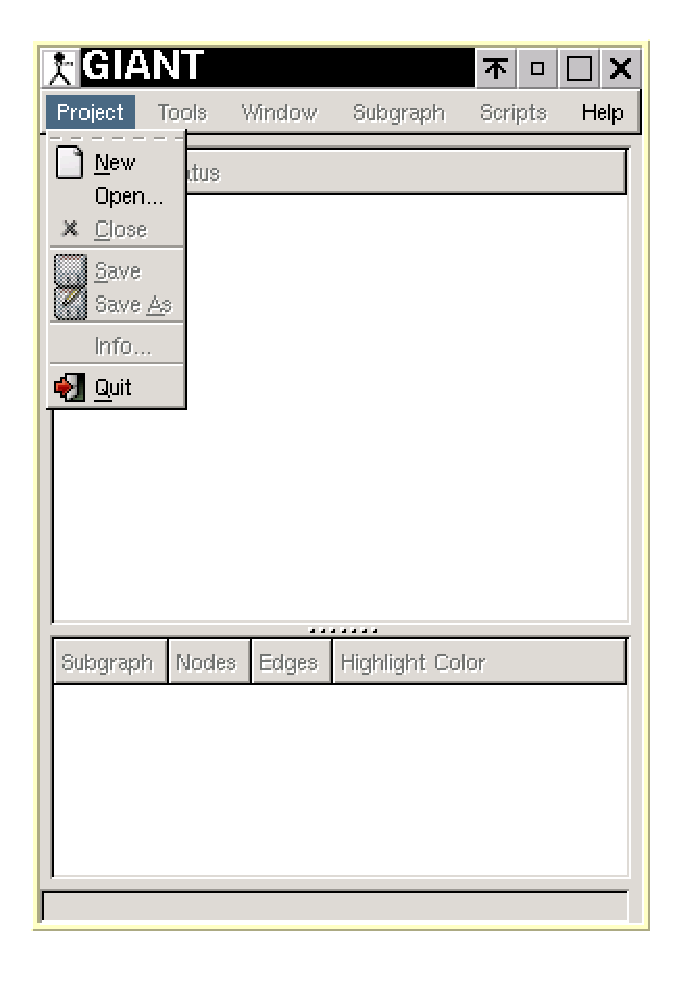
\includegraphics[scale=.75]{tutorial/01-a-main-project-menu}
   \caption{Main-Window}
\end{figure}

\clearpage


GIANT verlangt �ber den Dateiauswahl-Dialog nach Pfad und Namen
der neu zu erstellenden Projektdatei. Wir w�hlen hier\\
�/projects/tmp/birdy/giant-1.1.0/first_example/first_example�.\\
Dann fragt GIANT
durch einen Dateiauswahl-Dialog nach dem IML-Graphen, auf dem das
Projekt basieren soll. Wir w�hlen hier\\
�/projects/tmp/birdy/giant-1.1.0/graphs/rfg_examp.xml�.\\

GIANT meldet nun auf der Statuszeile links unten \gq{Project Initialized},
rechts unten steht der Name der IML-Datei, �rfg_examp.iml�.\\

\begin{figure}[h!]
   \centering
   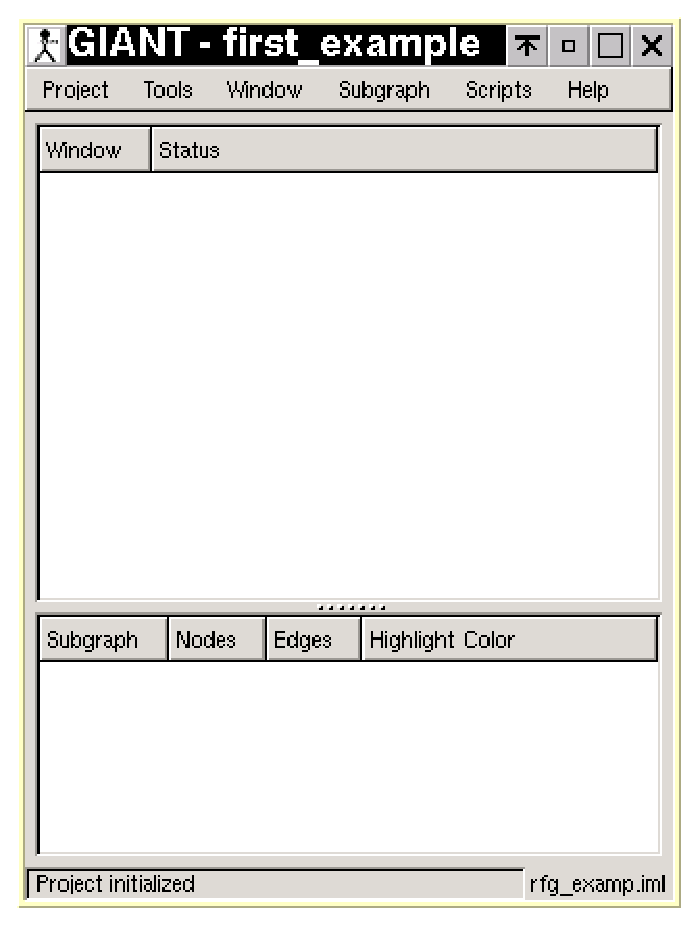
\includegraphics[scale=.75]{tutorial/02-main-project-loaded}
   \caption{Main-Window Bild 2}
\end{figure}

\clearpage

\section{�ffnen eines Fensters}

Wir wollen nun ein erstes Graphenfenster �ffnen. Das erledigen wir durch
Ausw�hlen des Men�punkts �Open Entire Graph� unter �Scripts�.\\

Nun erscheint ein Graphenfenster.

\begin{figure}[h!]
   \centering
   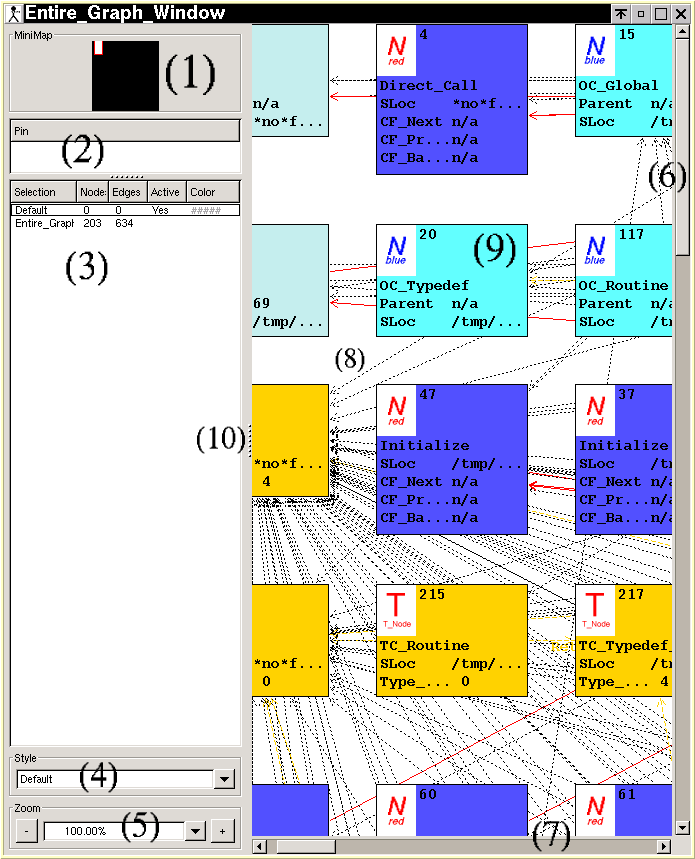
\includegraphics[scale=.5]{tutorial/03-entire-graph-window}
   \caption{Graphenfenster}
\end{figure}

\section{Zoomen}

Mittels der Zoomkontrolle (4) k�nnen wir die Ansicht im Fenster vergr��ern
oder verkleinern. Dazu k�nnen die Buttons �+� und �-� verwendet werden,
mittels der Combobox voreingestellte werte gesetzt werden oder ein
Wunschwert per Tastatur eingetragen werden. Wir tragen �45.00� Prozent
ein (und dr�cken Return), um einen guten �berblick zu erhalten.\\
Wir w�hlen eine beliebige Kante mit der linken Maustaste an und
w�hlen �Zoom to Edge�, worauf GIANT so scrollt und zoomt, da�
diese Kante komplett auf dem Bildschirm sichtbar ist.
Wir tragen nun wieder 45% als Zoomwert ein und dr�cken Return.

\section{Scrollen im Fenster}

Nun wollen wir den sichtbaren Anzeigeinhalt verschieben. Dies geht
durch Verschieben des wei�en K�stchens in der MiniMap (1) mit der Maus.
Wir verschieben das K�stchen ganz in die linke obere Ecke,
wo wir einige Knoten sehen k�nnen.\\

Selbstverst�ndlich kann die Fenstergr��e in der von anderen Programmen
gewohnten Weise ver�ndert werden. Zus�tzlich kann die Breite der linken
H�lfte des Fensters durch ziehen von Element (10) ver�ndert werden.
Durch Bet�tigen der Scrollbars (6) und (7) kann wiederum der sichtbare
Anzeigeinhalt verschoben werden.

\section{Knoteninformation anzeigen}

Wir suchen nun durch zoomen und scrollen den Knoten mit der Nummer 10,
welcher sich links Oben im Block der Knoten befindet (es kann auch ein
beliebiger anderer Knoten verwendet werden). Durch Klick
mit der rechten Maustaste auf den Knoten erscheint ein Popup-Men�, wir
w�hlen \gq{Show Info}. Es werden hier einige Informationen zum Knoten
angezeigt (Bild \ref{Node-Info Fenster}).
Durch Klicken von \gq{Pick} und Klick auf einen anderen Knoten kann
nunmehr die Information dieses anderen Knoten angezeigt werden.

\begin{figure}[h!]
   \centering
   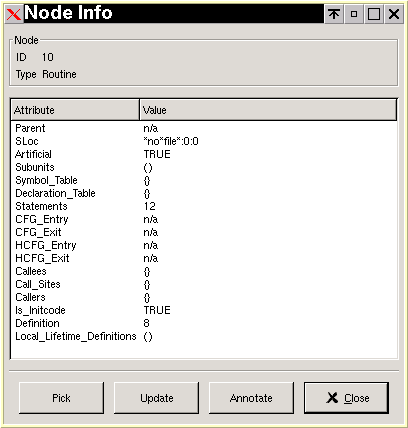
\includegraphics[scale=.4]{tutorial/04-nodeinfo}
   \caption{Node-Info Fenster}
   \label{Node-Info Fenster}
\end{figure}

Wir schlie�en das Nodeinfo-Fenster wieder.

\section{Pin festlegen / �ndern / l�schen}

Wir wollen uns nun eine Ansicht des Graphen f�r ein sp�teres schnelles Wiederfinden
merken. Dazu scrollen und zoomen wir in eine f�r uns interessante Position (z.B.
auf Knoten 176 rechts oben im Graphen), klicken mit der rechten Maustaste auf
eine wei�e Fl�che in der Ansicht und w�hlen im Men� \gq{New Pin...} an.
Bei der Frage nach dem Namen des Pins geben wir als Namen z.B. �Kn-176� ein.
Wenn wir nun in eine andere Position scrollen und zoomen, k�nnen wir
durch Aktivieren von �Show� im Popup-Men�, welches bei Auswahl des Knotennamens
mit der Rechten Maustaste in der Pinliste (2) erscheint, wieder zu genau
dieser Ansicht zur�ckspringen.\\
Mit �Rename...� kann der Name des Knotens ge�ndert werden. Wir �ndern den
Knotennamen auf �Interessanter_Knoten�.
Falls wir den Knoten sp�ter einmal l�schen wollen, geht dies mit �Delete�
im Kontextmen�.

\section{Visualisierungsstile �ndern}

Mittels der Visualisierungsstil-Auswahl (4) k�nnen wir die Art der Darstellung
der Knoten �ndern. Probeweise �ndern wir die Darstellung in der Combobox einmal
auf �Plain�. Wir k�nnen nun einmal im Graph herumzoomen und scrollen, um
die Unterschiede zu sehen.
Nun wechseln wir aber wieder zur�ck zum Default-Stil.

\section{Selektionen bearbeiten und markieren}

Wir springen nun zu unserem Pin �Interessanter Knoten�, und zoomen und
scrollen ggf. so, da� wir ca. 8 Knoten bei einer
Zoomstufe von 70 Prozent auf dem Bildschirm haben.\\

Nun klicken wir auf den Knoten Nr. 176 (rechts oben
in der Matrix) mit der linken Maustaste.\\

Der Knoten wird farbig markiert. Wir k�nnen sehen, da� in der Selektionsliste
(3) in der Zeile �Default� der angew�hlte Knoten auftaucht.
Mit gedr�ckter Shift-Taste w�hlen wir noch zwei andere Knoten aus.
Nun halten wir die Shift-Taste und ziehen mit gedr�ckter linker Maustaste
einen Rahmen �ber alle bis auf die unteren zwei Knoten.
Wenn wir loslassen, k�nnen wir feststellen, da� GIANT den momentanen
Status (Selektiert oder nicht) aller Knoten im Rahmen umgekehrt hat.\\

Wenn wir einen Rahmen ohne gedr�ckte Tasten ziehen, werden alle bisherigen
Knoten in der Default-Selektion entselektiert. Wir ziehen nun einen Rahmen
�ber die oberen beiden Knoten. Diesen wollen wir nun die unteren beiden
Knoten hizuf�gen. Dies geschieht durch Anklicken dieser beiden Knoten mit
gedr�ckter Shift-Taste. Alternativ k�nnte auch ein Rahmen mit gedr�ckter
Shift-Taste gezogen werden.\\

Nun ziehen wir einen Rahmen mit der Maus �ber alle Knoten im Fenster
bei gedr�ckter Ctrl-Taste. Wir k�nnen sehen, da� GIANT hier alle
Knoten im Rahmen markiert, im Gegensatz zur Umkehrung des Selektionsstatus
bei Verwendung der Shift-Taste.\\

Zu guter Letzt ziehen wir nochmals einen Rahmen ohne gedr�ckte Tasten �ber
die oberen vier Knoten.\\

Das Selektieren von Kanten funktioniert v�llig analog zum Selektieren der
Knoten.\\

Durch den Rahmen haben wir nun eine gewisse Anzahl von Knoten und Kanten
in der Default-Selektion sichtbar in (3).
Wir duplizieren nun diese Auswahl durch Ausw�hlen von �Duplicate� im Kontextmen�
nach Dr�cken der rechten Maustaste �ber �Default� in der Selektionsliste (3).
Als Namen w�hlen wir �Neu�.\\

Nun wollen wir die Selektion �Neu� farbig markieren. Wir w�hlen dazu in
(3) im Kontext-Men� dieser Selektion �Highlight - Color 1� an.
Wir k�nnen nun sehen, da� die Selektion farbig markiert wurde. (Siehe Bild \ref{Graphenfenster mit rot hervorgehobenem Graph})\\

Durch Ausw�hlen von �Select All� oder �Select Nothing� bei Rechtsklick auf ein
St�ck von Knoten oder Kanten leeren Hintergrund des Anzeigefensterinhaltes k�nnen
alle Knoten und Kanten markiert oder entmarkiert werden.\\

\begin{figure}[h!]
   \centering
   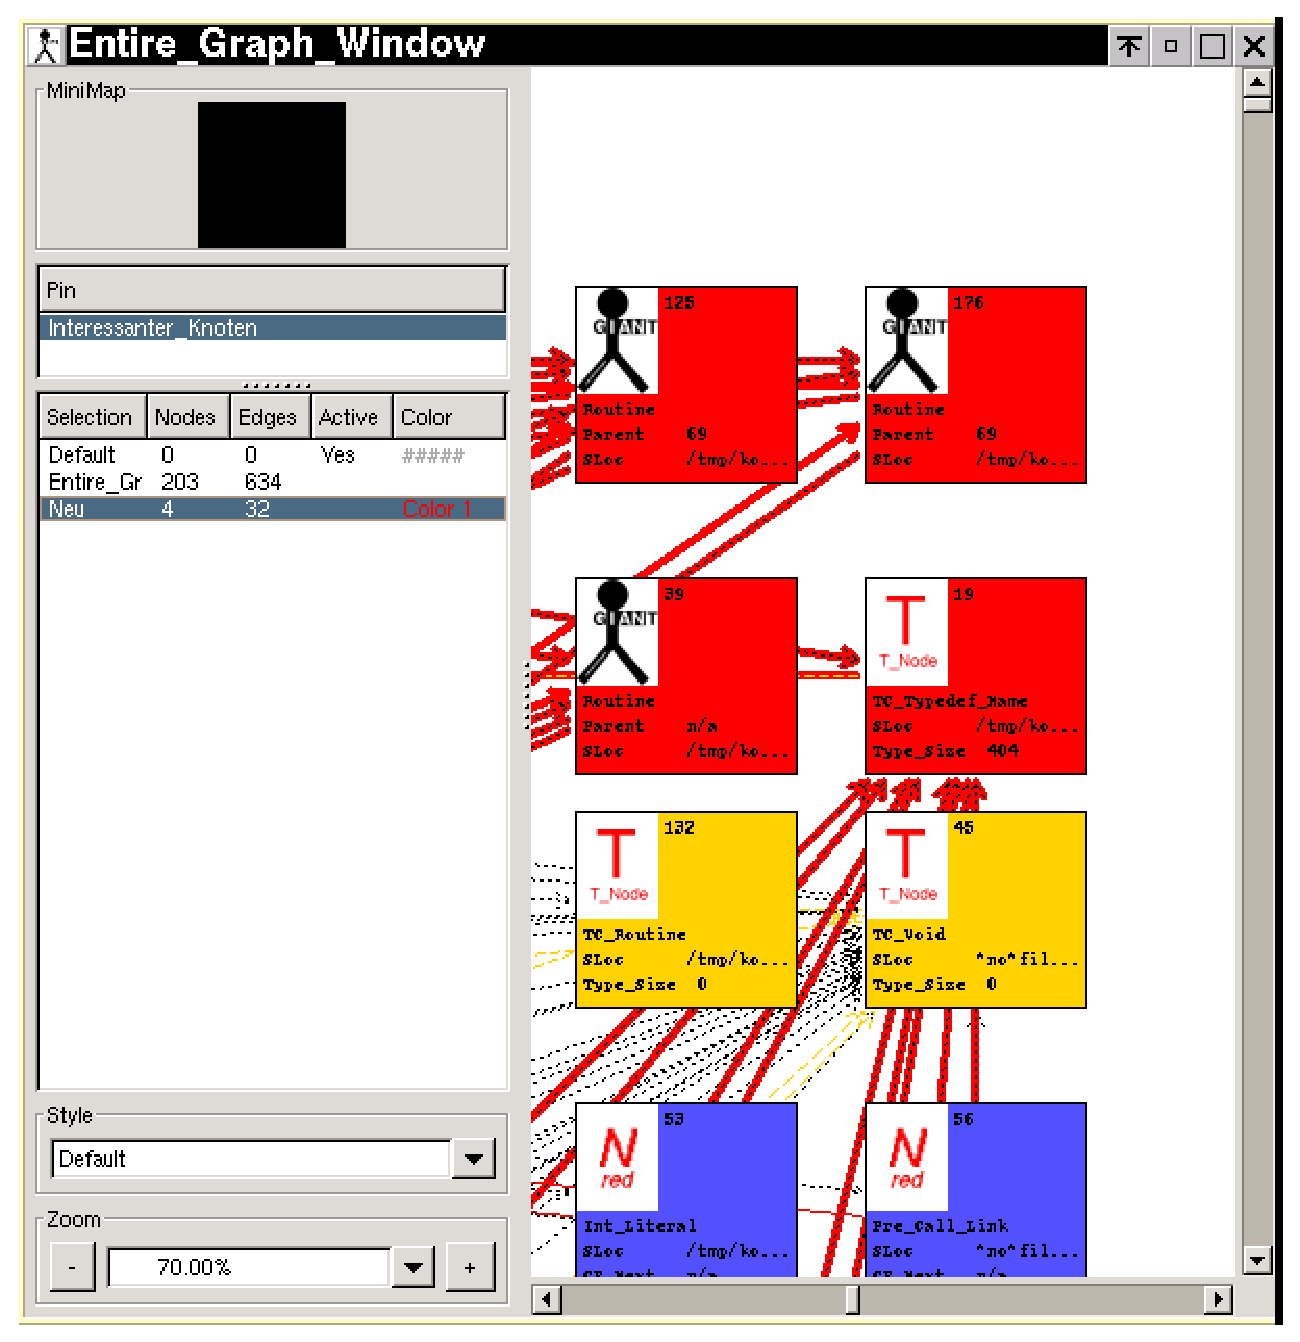
\includegraphics[scale=.5]{tutorial/05-selection-color}
   \caption{Graphenfenster mit rot hervorgehobenem Graph}
   \label{Graphenfenster mit rot hervorgehobenem Graph}
   \clearpage
\end{figure}

Wenn wir nun im Kontextmen� der Selektion �Zoom to Selection� ausw�hlen,
zoomt und scrollt GIANT so in den Graph hinein, da� alle Knoten der
Selektion sichtbar sind.\\

Mit unserem neu erworbenen Wissen erstellen wir nun eine Selektion
mit der Vierergruppe Knoten unten rechts im Graphen und nennen
sie �vier�. Nun w�hlen wir im Kontextmen� dieser Selektion
�Delete� aus und wir sehen, da� die Knoten noch da sind, die Selektion
aber gel�scht wurde.
Nun erstellen wir nochmals eine Selektion mit dem Namen �neu2�,
w�hlen diesmal �Delete with Content� aus.
GIANT hat nun die Knoten nebst ihrer Kanten aus dem Graph gel�scht.\\

Nun zu einer Mengenoperation:
Auf der Selektion �Neu� in (3) w�hlen wir nun �Set Operation� aus.
Es erscheint der Set Operation Dialog. Wir w�hlen
(siehe Bild \ref{Set Operation Dialog f�r Mengenoperationen}) \\

�Left Source = Entire_Graph�\\
�Operation = Difference�\\
�Right Source = Neu�\\
�Target = Differenzmenge�\\
aus.

\begin{figure}[h!]
   \centering
   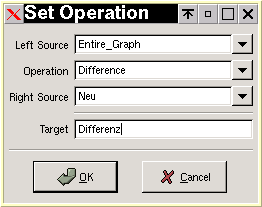
\includegraphics[scale=.5]{tutorial/06-set-operation}
   \caption{Set Operation Dialog f�r Mengenoperationen}
   \label{Set Operation Dialog f�r Mengenoperationen}
\end{figure}
\clearpage

Nun bildet GIANT die Differenz zwischen den beiden Mengen �Entire_Graph�
(also dem Gesamtgraphen) und der Menge �Neu�, die neue Menge heisst
�Differenzmenge�. Man kann sehen, wie sich die Kantenzahlen
unterscheiden.\\
Nun w�hlen wir auf �Differenzmenge� den Men�punkt �Set Active� aus.
Diese Menge ist nun die aktive Selektion. 
Wir k�nnen nun sehen, da� alle Knoten im Graphen, die zur Menge
geh�ren, markiert sind. Mit gedr�ckter Shift-Taste k�nnen wir nun
z.B. Knoten zur Selektion hinzuf�gen oder aus ihr entfernen.

Nachdem wir einige Knoten ausgew�hlt haben, w�hlen wir wieder die
�Default� Selektion als Aktiv an.\\

Unsere Sekektion �Differenzmenge� mit ihren ausgew�hlten Knoten
f�gen wir nun als eigenst�ndigen Subgraphen in GIANT ein, dies
passiert durch Ausw�hlen von �Insert as Subgraph� in ihrem
Kontextmen�. Wie wir sehen, erscheint sie nun im Hauptfenster
in der Subgraph-Liste.\\

\section {Verschieben von Knoten, Platz schaffen}

Wir k�nnen mit der linken Maustaste durch Drag and Drop Knoten
verschieben. Es kann vorkommen, da� Knoten aufeinander liegen,
sie k�nnen dann damit auseinandergeschoben werden.\\

Durch Klick mit der rechten Maustaste auf einen freien Platz im
Anzeigeinhalt des Graphenfensters k�nnen wir im Popup-Men�
�Make Room� anw�hlen. Durch diese Operation werden die
Knoten rund um den freien Platz auseinandergeschoben, je n�her
desto weiter. Bild \ref{Make-Room-Result} zeigt das Ergebnis einer
solchen Operation.

\begin{figure}[h!]
   \centering
   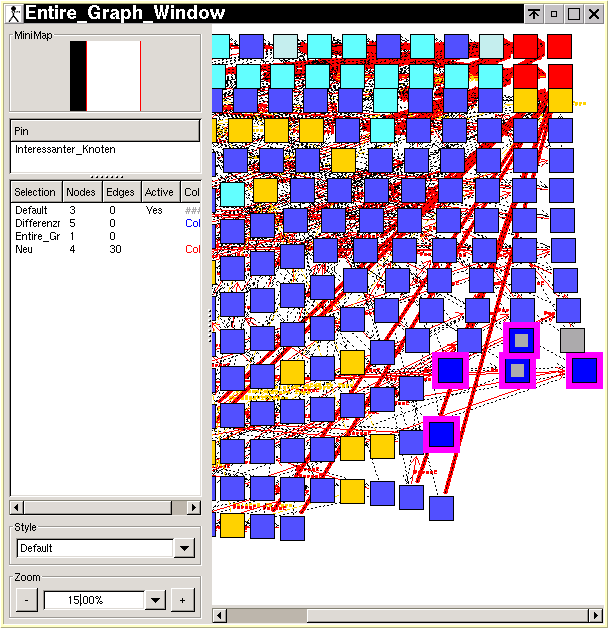
\includegraphics[scale=.5]{tutorial/08-make-room}
   \caption{Resultat von Platz schaffen}
   \label{Make-Room-Result}
\end{figure}


\section{Mehrere Fenster}

Durch Ausw�hlen von �Window - New� erschaffen wir ein neues leeres
Fenster. Dieses wird in der Fensterliste im Hauptfenster angezeigt.
Das Fenster heisstr �Unknown�, wir �ndern seinen Namen durch
Anw�hlen von �Rename� auf im dazugeh�rigen Popup-Men� in der
Liste auf �Testfenster�.\\
Wir schlie�en nun unser eingangs erstelltes Fenster �Entire_Graph_Window�
durch Klick auf den Close-Button rechts oben und speichern es bei der
erscheinenden Sicherheitsabfrage.
Mittels �Open� in seinem Popup-Men� k�nnen wir es bei Bedarf wieder �ffnen.\\

\begin{figure}[h!]
   \centering
   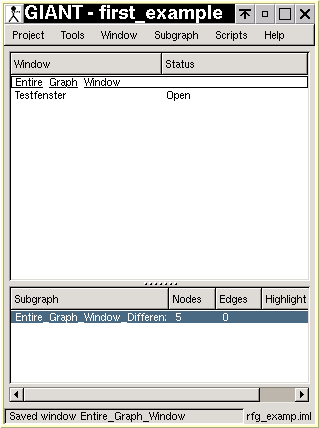
\includegraphics[scale=.5]{tutorial/07-main-window}
   \caption{Hauptfenster}
\end{figure}

Nun wollen wir unseren Teilgraphen in das neue Testfenster einf�gen.
Dazu w�hlen wir im Hauptfenster auf dem erstellten Subgraphen im
Popup-Men� �Insert as Selection�. GIANT fordert uns auf, in den leeren
Anzeigeinhalt des Fensters zu klicken, dort wird der Subgraph als Selektion
eingef�gt.\\

Wir �ffnen nun wieder unser erstes Fenster �Entire_Graph_Window�durch
Ausw�hlen von �Open� auf seinem Popup-Men�.\\

Wir w�hlen im Kontextmen� des Subgraphen im Hauptfenster aus\\
�Highlight - Color 2� und k�nnen sehen, da� unsere
Selektion in beiden Fenstern hervorgehoben wurde. Mittels
�Unhighlight in alle Windows� l��t sich die Markierung r�ckg�ngig
machen.\\

Wir schlie�en und speichern das �Testfenster�.

\section{Layouts}

Mittels des oben erw�hnten �Select All� entmarkieren wir alle Knoten in
unserem verbleibenden Fenster. Wir sorgen daf�r, da� im Fenster ca.
die H�lfte des Anzeigeinhaltes frei ist.
Wir w�hlen durch Ziehen mit der Maus ca. 10-15 Knoten im linken
oberen Teil des Graphen aus und w�hlen
dann in der Selektionsauswahlliste auf der aktiven �Default� Selektion
�Apply Layout� aus.\\


Mittels �Matrix Layout� l��t sich der Inhalt des Fensters in
eine Matrixform bringen. Wir w�hlen diese Option im Tab aus
(siehe Bild \ref{Matrix-Layout}).

\begin{figure}[h!]
   \centering
   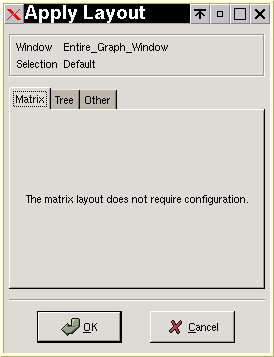
\includegraphics[scale=.6]{tutorial/09-matrix-layout}
   \caption{Apply Layout}
   \label{Matrix-Layout}
\end{figure}

Nach Klick auf �OK� klicken wir an eine leere Stelle im Anzeigefenster-
Inhalt, dies zeigt GIANT, wo die umorganisierten Knoten platziert
werden sollen.
Ein m�gliches Resultat wird in Bild \ref{Matrix-Layout2} gezeigt.

\begin{figure}[h!]
   \centering
   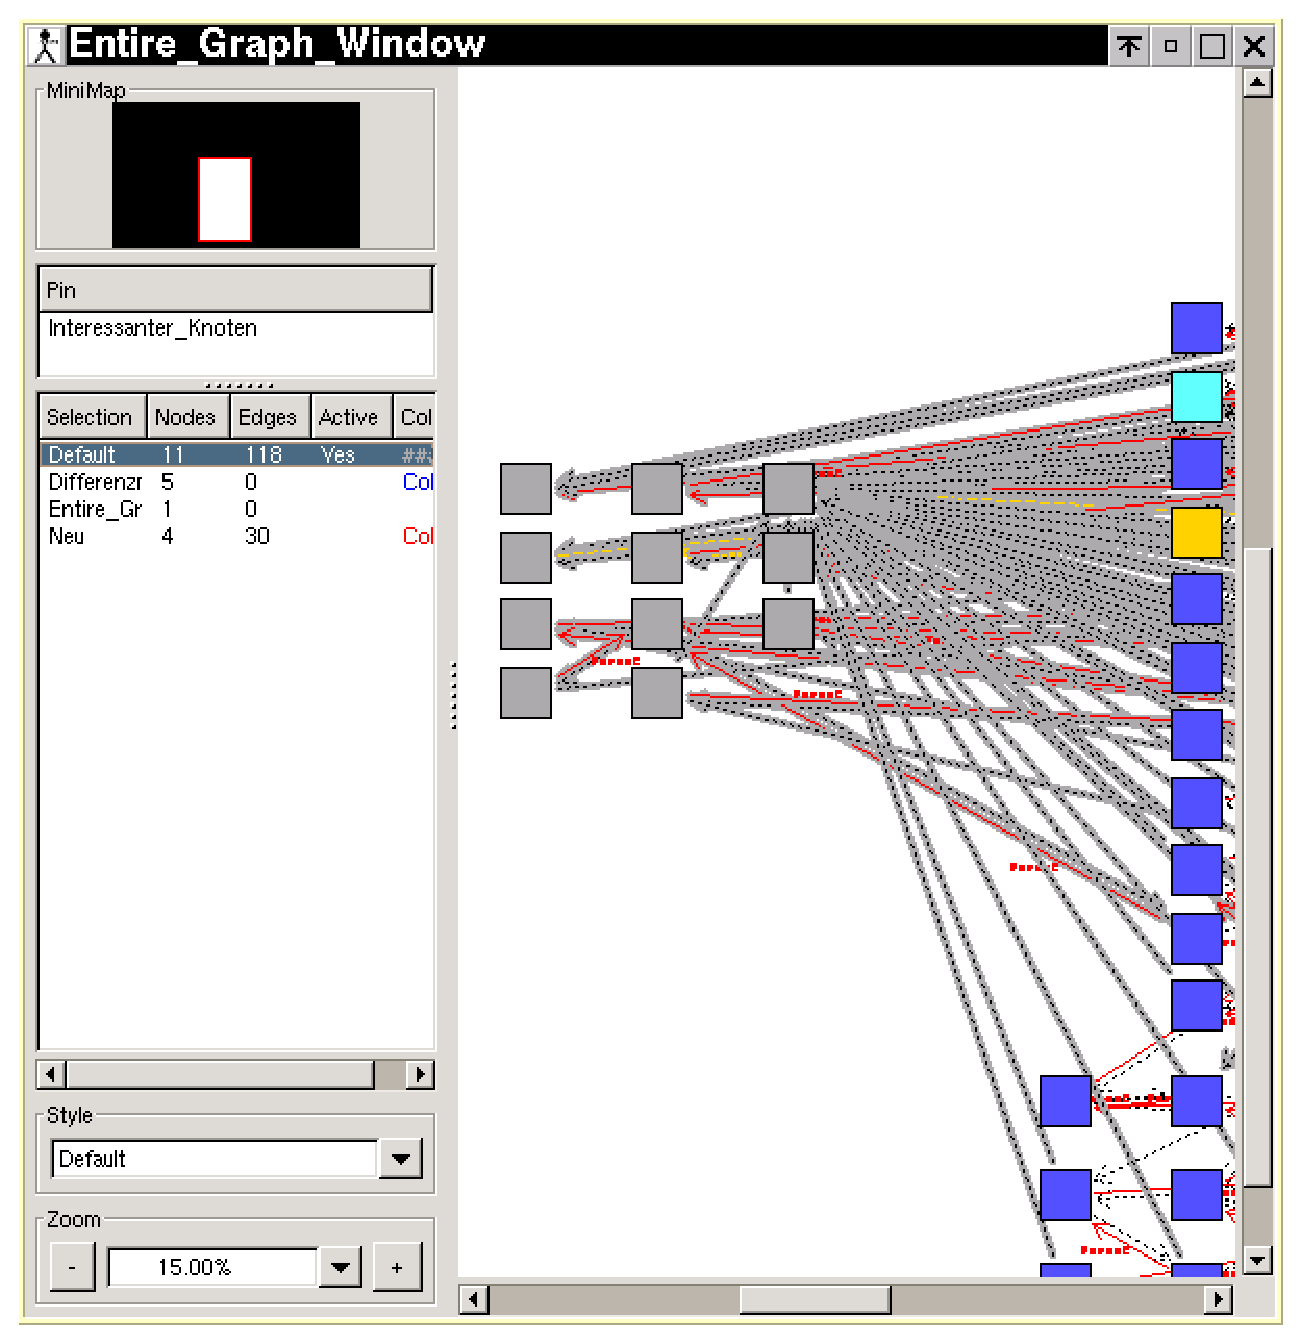
\includegraphics[scale=.55]{tutorial/10-matrix-layout2}
   \caption{Ergebnis des Matrix-Layouts}
   \label{Matrix-Layout2}
\end{figure}


Wir w�hlen im Popup-Men� des Knoten rechts oben �Show Info�
aus und merken uns den oben im Fenster angezeigten numerischen Wert �ID�
des Knotens.

Nun w�hlen wir ca. 5 * 5 Knoten in der rechten oberen Ecke des Graphen
durch Ziehen mit der Maus aus, einer dieser Knoten sollte der mit der
bekannten ID sein. Vorher sollten wir daf�r sorgen, da�
auch noch gen�gend freier Platz im Fenster sichtbar ist.\\



Wir w�hlen dann in der Selektionsauswahlliste auf der aktiven �Default�
Selektion �Apply Layout� aus. In das Feld �Root Node ID� tragen wir
die ID des Knotens ein.
In der Liste �Class Sets� w�hlen wir �parent_edge_class_set�, �empty_class_set�
und �normal_class_set� aus. Dies sind die Klassenmengen, die f�r das
Layout ber�cksichtigt werden. Nun ist noch ein Klick an die Position
des Wurzelknotens im Anzeigefenster n�tig, und das Layout wird berechnet
und angezeigt.

% **** Kein Bild hier, weil Bug - es wird ein Matrixlayout berechnet!

\section{Benachbarte Knoten}

Mittels des Men�punktes �Scripts - Get Adjacent Nodes� k�nnen die
benachbarten Knoten eines Knotens in eine Knotenmenge eingef�gt werden.

% **** Kein Bild, weil GSL Errors.

%\section{Search for Routine}
%
%Durch Auswahl von �Scripts - Search for Routine� kann mit Wildcards
%**** ja was eigentlich?

\section{Annotieren}

Knoten k�nnen durch Klick auf �Annotate� im Knoteninformationsfenster
(siehe Bild \ref{Node-Info Fenster}) oder durch Auswahl des Punktes
�Annotate� im Knoten-Popup-Fenster annotiert werden.

Nach der Auswahl von �Annotate� �ffnet sich das Knoten-Annotationsfenster
(siehe Bild \ref{Node Annotation Window}). Hier kann ein Kommentar zum
Knoten eingef�gt werden, der mit gespeichert wird. Durch Delete
kann der Kommentar wieder gel�scht werden.

\begin{figure}[h!]
   \centering
   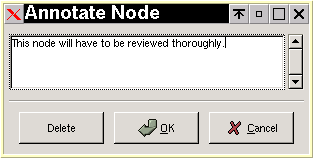
\includegraphics[scale=.55]{tutorial/11-annotation}
   \caption{Knoten-Annotationsfenster}
   \label{Node Annotation Window}
\end{figure}

Nach dem Annotieren wird der Benutzer bei gen�gend gro�er Zoomstufe
durch ein kleines \gq{Dokument}-Symbol auf die Annotation
aufmerksam gemacht. (siehe Bild \ref{Node Annotation Window2})

\begin{figure}[h!]
   \centering
   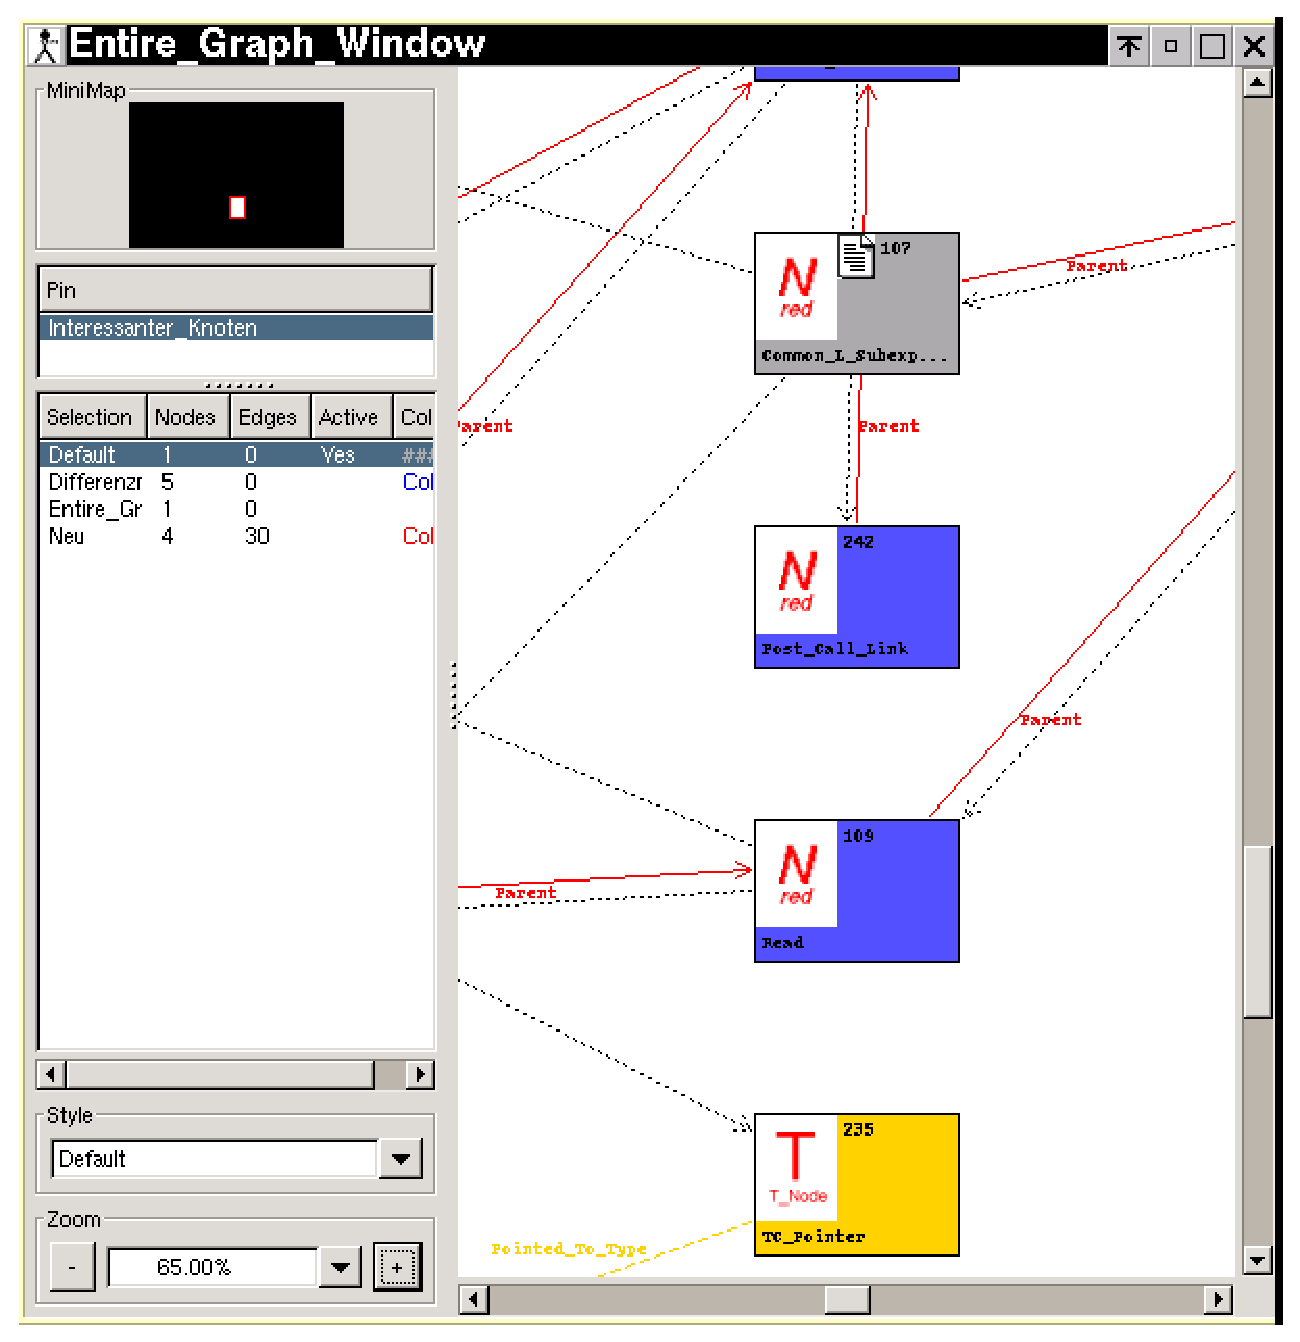
\includegraphics[scale=.55]{tutorial/12-annotation2}
   \caption{Annotierter Knoten Nr. 107}
   \label{Node Annotation Window2}
\end{figure}



%===============================================================================
% 
% Beschreibung der Funktionen
%
\chapter{Beschreibung der Benutzeroberfl�che}
\label{Beschreibung der Funktionen}

Dieses Kapitel beschreibt, geordnet nach den in GIANT auftretenden Fenstertypen,
alle Buttons, Men�s und Funktionen. Dies ist als Nachschlagewerk �ber
alle Elemente der graphischen Benutzeroberfl�che (GUI) gedacht.

% ==============================================================================
%  $RCSfile: functions.tex,v $, $Revision: 1.24 $
%  $Date: 2003/10/07 14:30:22 $
%  $Author: koppor $
%
%  Description: 
%
%  Last-Ispelled-Revision:
%
% ==============================================================================

\label{Kapitel-Funktionale Anforderungen}

%\section{�ber dieses Kapitel}    
%
%
%Wichtige Informationen zur Persitzenz der Projekte in GIANT,
%welche Informationen jeweils gespeichert werden, finden sich
%im Abschnitt \ref{Project Persistenz der Projekte}.

\section {Kommandozeilenaufruf} \label{fa Starten von GIANT}

Giant kann wie folgt von der Kommandozeile aus gestartet werden:

\begin{enumerate}
 \item{Ohne Parameter:}\\

�./giant�

 \item{Mit Parametern, �[]� bedeutet \gq{optional}, �|� bedeutet \gq{oder}:}\\

�./giant  project-file [-g graph-file] [-e script-file]�\\
�     [-c config-file] | -h | -v�

�project-file� ist der Filename der Projektdatei, �graph-file� der Filename
des IML-Graphen. �script-file� ist eine Datei, die ein GSL Script enth�lt,
da� nach dem Laden bzw. Erzeugen des Projektes Ausgef�hrt wird. �config-file�
ist die optional anzugebende globale Konfigurationsdatei, siehe Abschnitt
\ref{config-allgemeines-punkt2}.

Die Option �-h� steht f�r Hilfe, mit �-v� kann die Programmversion von
GIANT angezeigt werden.\\
Wenn ein Graph-File angegeben wird und �project-file� nicht existiert, wird
ein neues Projekt mit diesem Namen erzeugt.\\

Ein Beispiel f�r den Kommandozeilenaufruf von GIANT ist:\\

�./giant projects/sample.project -g graphs/mygraph.xml�\\

\end{enumerate}

\clearpage
\section {Main Window}

\begin{figure}[h!]
   \centering
   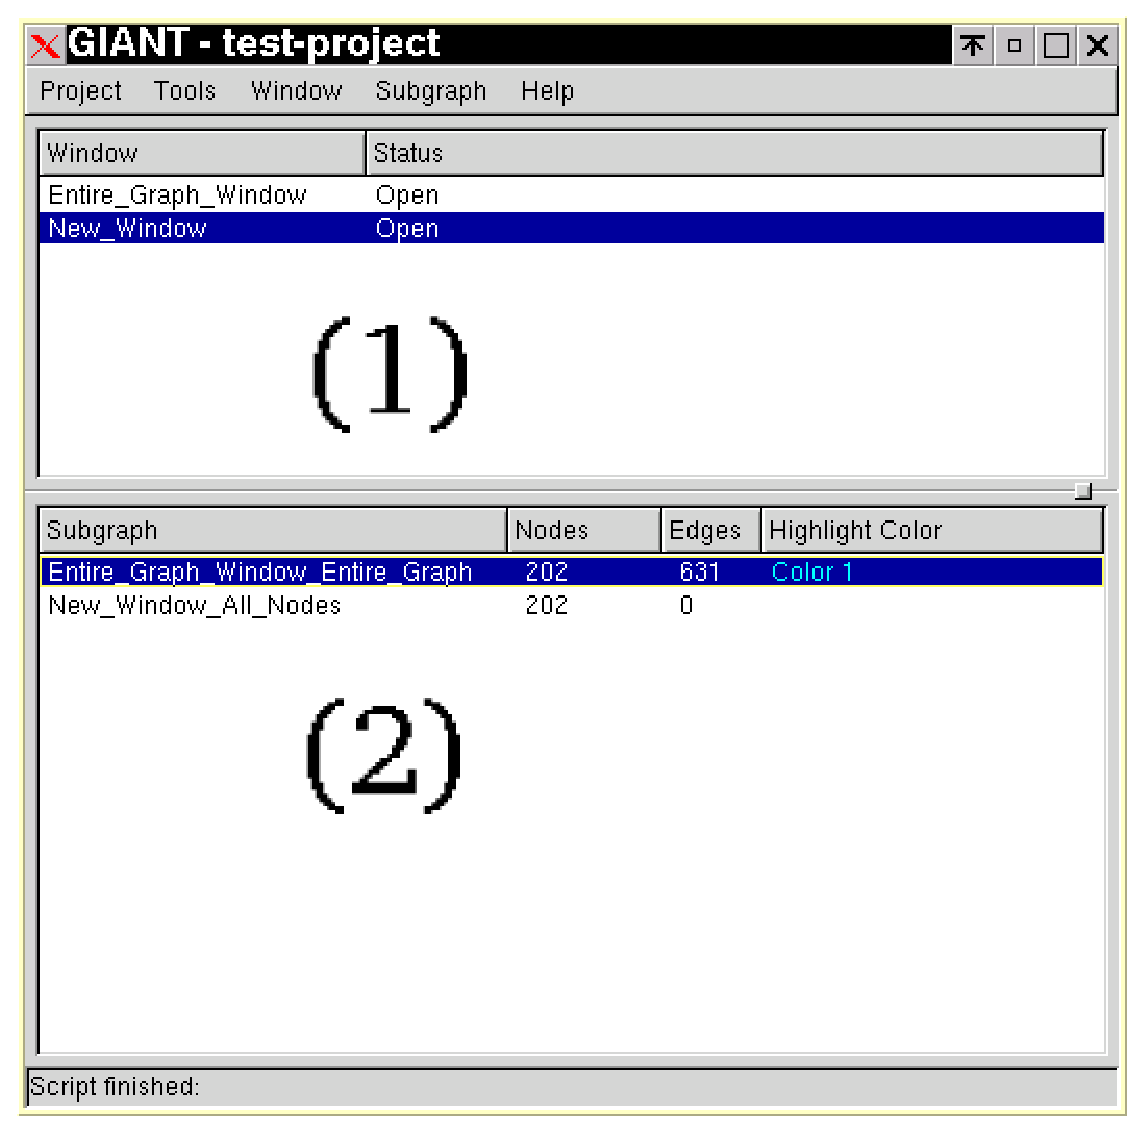
\includegraphics[scale=.75]{gui/main_window}
   \caption{Main-Window}
   \label{Main-Window-Pic}
\end{figure}

\clearpage

%Erg�nzungen by Martin
Jede Instanz von GIANT hat genau ein Hauptfenster. \index{Hauptfenster}
Im Hauptfenster (siehe Abbildung \ref{Main-Window-Pic}) werden die
Anzeigefenster und
IML-Teilgraphen des aktuell ge�ffneten Projektes (siehe  
\ref{Project Persistenz der Projekte}) in Listen angezeigt. 
�ber Popup-Men�s k�nnen IML-Teilgraphen
und Anzeigefenster manipuliert werden.

Im Fenster befinden sich zwei Listen, Window List (1) und
Subgraph List (2).


  \subsection {Titelzeile}
  In der Titelzeile wird \gq{GIANT - <Projektname>} dargestellt.
 
  \subsection {Men�leiste (Main Window)}
  In der Men�leiste befinden sich folgende Eintr�ge:

    \subsubsection {Untermen� Project} \label{Main-Window-Project}
      \begin{enumerate}
         \item {New}\\
         
         Hiermit wird ein neues Projekt angelegt. Ein eventuell bereits ge�ffnetes
         Projekt wird dabei geschlossen, wobei �nderungen auf Nachfrage 
         vorher gespeichert werden.

         \begin{itemize}
         
    \item{GIANT zeigt den Standard-Filechooser-Dialog und fordert den
    Benutzer auf, eine vorhandene IML-Graph Datei auszuw�hlen.}
    
    \item{GIANT zeigt erneut den Standard-Filechooser-Dialog und fordert den
    Benutzer zur Eingabe des Namens der Projektdatei auf. Die Dateiendung wird sp�ter
    von GIANT automatisch gesetzt.}
    
    \item {Der Name der Projektdatei ist
    automatisch auch der Name f�r das Projekt. Das Verzeichnis der
    Projektdatei wird automatisch zum Projektverzeichnis. Existiert die eingegebene Projektdatei bereits, 
    erscheint eine Fehlermeldung.
    Existiert in dem Projektverzeichnis bereits eine andere Projektdatei, so 
    erscheint ebenfalls eine Fehlermeldung.}
        \end{itemize}
    
         \item {Open}\\
         
         �ffnet ein GIANT Projekt. Ein eventuell bereits ge�ffnetes
         Projekt wird dabei geschlossen, wobei �nderungen auf Nachfrage 
         vorher gespeichert werden.
         \begin{itemize}
           \item {War vorher bereits ein Projekt offen, erscheint vorher eine
           Abfrage, ob dieses gespeichert werden soll.}
           \item {GIANT zeigt den Standard-Filechooser-Dialog und fordert
           den Benutzer zur Auswahl einer vorhandenen GIANT-Projektdatei auf.}
         \end{itemize}
         \item {Save}
         
         Speichert ein Projekt in die Verwaltungsdateien im Projektverzeichnis
         der neuen Projektdatei.
         
         \item {Save As...}
         
         Speichert ein Projekt in die Verwaltungsdateien im Projektverzeichnis
         der neuen Projektdatei unter neuem Namen.
         
         \begin{itemize}
          \item{Der Benutzer gibt im Standard-Filechooser-Dialog 
             das neue Projektverzeichnis 
             und den Namen f�r die neue Projektdatei ein, die Dateiendung 
             wird sp�ter von GIANT automatisch gesetzt.}
         \end{itemize}
         
         \item {Info}
         
         Zeigt einen Informationsdialog �ber den Graphen an.
         
         \item {Quit}
         
         Beendet das Programm GIANT.
         
      \end{enumerate}    
      
     \subsubsection {Untermen� Tools}  \label{Main-Window-Tools}
       \begin{enumerate}

          \item {GSL Editor...}
          
          Mit diesem Men�punkt kann ein GSL Script ausgef�hrt werden.
          Es erscheint der Skriptdialog, in den das Skript eingegeben
          werden kann. Es ist auch m�glich, Skripte zu laden oder zu
          speichern. Details hierzu finden sich unter \ref{GUI Anfragedialog}.
          
        \end{enumerate}
        
        
    \subsubsection {Untermen� Window}  
        \begin{enumerate}
          \item {New}\\
          Mit diesem Men�punkt kann ein neues leeres Fenster ge�ffnet werden.
        \end{enumerate}
    \subsubsection {Untermen� Subgraph}  
        \begin{enumerate}
          \item {New}\\
          Mit diesem Men�punkt kann ein neuer leerer IML-Teilgraph erstellt werden.
         \item {Set Operation}\\
          Mit diesem Men�punkt kann eine Mengenoperation auf IML-Teilgraphen
          durchgef�hrt werden, GIANT zeigt dazu den \gq{Set Operation Dialog},
          siehe Abschnitt \ref{Common-Set-Operation-Dialog}.
        \end{enumerate}
        

    \subsubsection {Untermen� Help}  \label{Main-Window-Info}     
       \begin{enumerate}
          \item {About..}\\
          Dieser Men�punkt gibt ein Fenster mit Informationen zur
          GIANT Programmversion und zu den Autoren aus.
        \end{enumerate}
     

  \subsection {Statuszeile}
  \label{Statuszeile}
  \index{Statuszeile}
  Die Statuszeile befindet sich ganz unten im Hauptfenster. In der
  Statuszeile werden Informationen zum aktuellen Zustand von GIANT
  dargestellt.

   \subsection {Window List (1)}
  
   Im Hauptfenster befindet sich zuoberst eine Liste \gq{Window List}, welche
   alle Anzeigefenster des Projektes (offen und geschlossen anzeigt).
   Eine Beschreibung, was alles mit einem Fenster gespeichert wird,
   befindet sich in Abschnitt \ref{Project Persistenz der Projekte}.
   
   \subsubsection {Inhalt Window List}
   \label{WINDOW-LIST}
   
   Window List hat die Spalten \gq{Window} und \gq{Status}. In
   \gq{Window} wird der Name aller Anzeigefenster dargestellt, in
   \gq{Status} befindet sich der Text "Open", wenn das Fenster
   ge�ffnet ist.
    
    \subsubsection {Popup-Men� Window List}
    
    
        Beim Rechtsklick auf Window List �ffnet sich ein 
        Popup-Men� mit folgenden Men�punkten:
        \label{WINDOW-LIST-POPUP}

        \begin{enumerate}
          \item Open\\
             �ffnet ein im Speicher vorhandenes, momentan geschlossenes Fenster.
          \item Close\\
             Schlie�t ein vorhandenes Fenster, es kann wieder ge�ffnet werden.
             Falls das Fenster noch nicht gespeichert wurde, wird eine
             Sicherheitsabfrage durchgef�hrt, ob gespeichert werden soll.
          \item Save Window\\
             Speichert ein Fenster im Projektverzeichnis.
          \item Rename Window\\
             �ndert den Namen eines Fensters, ein entsprechender Dialog erscheint.
          \item Delete Window\\
             L�scht ein Fenster aus dem Projektverzeichnis, es wird auch aus der Window List gel�scht.
        \end{enumerate}
    
  \subsection {Subgraph List (2)}
  \label{GUI Subgraph List}
    
    Unter der Window List befindet sich eine Liste \gq{Subgraph List} mit
    allen IML-Teilgraphen des Projektes.
   
    \subsubsection {Inhalt Subgraph List} 
    
      Subgraph List hat die folgenden Spalten:
      \begin{enumerate}
        \item Subgraph
        \item Nodes
        \item Edges
        \item Color
      \end{enumerate}
    
      In der Spalte Name stehen die Namen der existierenden IML-Teilgraphen,
      in Nodes die Anzahl der Graph-Knoten des jeweiligen IML-Teilgraphen, 
      in Edges die Anzahl der Graph-Kanten und in Highlighted befindet sich
      ein K�stchen in der
      Farbe, die f�r die Hervorhebung des IML-Teilgraphen verwendet wird.
      Bei nicht hervorgehobenen IML-Teilgraphen wird dieses K�stchen
      nicht angezeigt.

    
    \subsubsection {Popup-Men� Subgraph List}
    \label {Popup-Men� Subgraph List}
      Bei einem Rechtsklick auf Subgraph List �ffnet 
      sich ein Popup-Men� mit folgenden Men�punkten:
        \label{SUBGRAPH-LIST-POPUP}
        \begin{enumerate}
          \item Highlight (Men�)
            \begin{enumerate}
              \item Color 1
              \item Color 2
              \item Color 3\\
              Mit diesen drei Men�punkten kann der angew�hlte IML-Teilgraph
              in allen Fenstern in der ausgew�hlten Farbe markiert werden.
            \end{enumerate}
          \item Unhighlight In All Windows\\
             Mit diesen drei Men�punkten kann der angew�hlte IML-Teilgraph
              in allen Fenstern wieder entf�rbt werden, die Markierung also
              entfernt werden.
              
              
          \item Insert as Selection\\
             Mit diesem Men�punkt kann ein IML-Teilgraph als Selektion in ein
             Fenster kopiert werden. Nach Ausw�hlen dieser Funktion ist mit der
             Maus (linke Taste) in das Fenster zu klicken, in das der Subgraph
             eingef�gt werden soll, an eine passende Stelle zu klicken.
          \item Rename
             Mit dieser Funktion kann der Name eines IML-Teilgraphen ge�ndert werden,
             ein entsprechender Dialog erscheint nach der Auswahl dieses Punktes.
          \item Duplicate
             Mit dieser Funktion kann ein IML-Teilgraph dupliziert werden,
             ein Dialog zur Auswahl eines neuen Namens erscheint nach der
             Auswahl dieses Punktes.
          \item Delete
             Mit diesem Men�punkt kann ein IML-Teilgraph nach Sicherheitsabfrage
             gel�scht werden.
        \end{enumerate}   
        Als weitere Men�punkte im Popup-Men� erscheinen die im GIANT-Config-File
        definierten kontextsensitiven GSL-Skripte. Mehr Informationen hierzu finden
        sich in Abschnitt \ref{Config-GSL-Context-Scripts}.

\clearpage
\section {Anzeigefenster} \label{GUI Anzeigefenster}
\index{Anzeigefenster}

  \begin{figure}[!htbp]
     \centering
     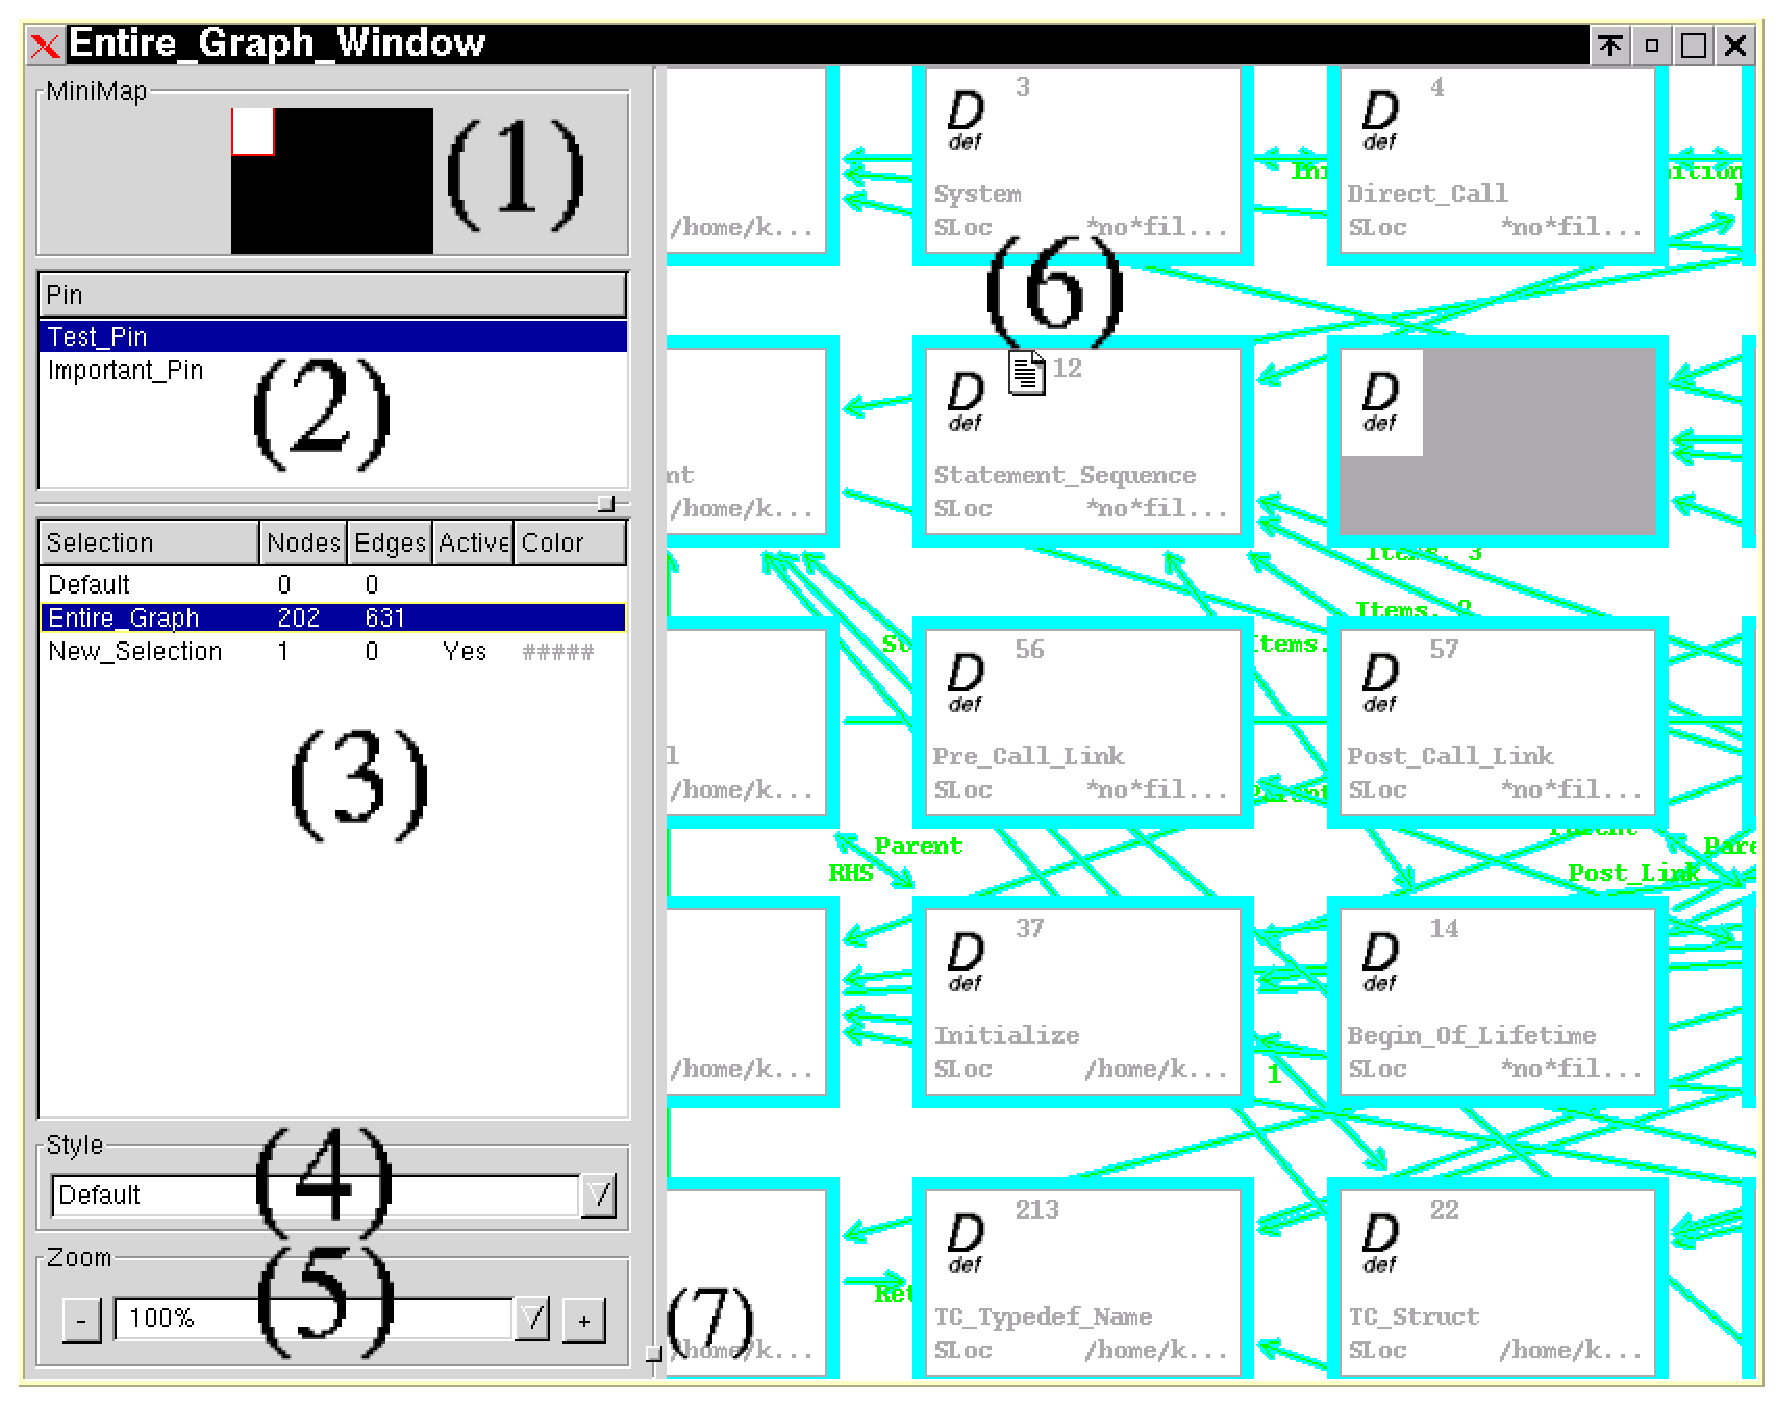
\includegraphics[width=16cm]{gui/visualization_window}
     \caption{Graph-Window}
     \label{Graph-Window-Pic}
  \end{figure}

  Im Programm kann es mehrere Anzeigefenster 
  (siehe Abbildung \ref{Graph-Window-Pic}) geben. 
  

  In Anzeigefenstern (Visualization Windows) werden Teile des IML-Graphen
  visualisiert.  Sie erscheinen im gro�en quadratischen rechten Teil
  (\gq{Vis Pane} (6)) des Fensters. Die Vis Pane enth�lt den Anzeigeinhalt
  des Fensters.  Im linken Teil des Fensters, der Toolbar
  (\gq{Vis Toolbar}) befinden sich untereinander die
  MiniMap (1), Pinliste (2), Selektionsliste (3), die Stilauswahl-Combobox (4) und die
  Zoom-Kontrolle (5). Dieser Teil kann durch Verschieben des entsprechenden
  Buttons (7) unten an der Trennleiste in der Gr��e ver�ndert werden.
  \index{Zoom-Kontrolle}
  \index{Visualisierungsstile!Stilauswahl-Combobox}

 \subsection {MiniMap (1)} \label{GUI Minimap}
 \index{Minimap} 
 
 In der MiniMap wird der Anzeigeinhalt verkleinert dargestellt,
 der Graph wird jedoch nur durch einen grauen Kasten repr�sentiert,
 Knoten sind nicht sichtbar. Die MiniMap wird von einem Rahmen
 umschlossen. Der sichtbare Anzeigeinhalt wird durch einen kleineren
 Rahmen repr�sentiert, der innerhalb der MiniMap durch Mausklicks
 versetzt werden kann. Je nach Zoomstufe ist dieser Rahmen gr��er
 oder kleiner. Wird der Rahmen versetzt, wird der sichtbare Anzeigeinhalt
 in der Vis Pane entsprechend angepasst.\\
 Vergr��ert sich die von Knoten bedeckte Fl�che im Fenster, z.B. durch
 Einf�gen von Teilgraphen, so ver�ndert sich auch die Minimap entsprechend.

  \subsection{Visualisierung der Knoten und Kanten (6)}

    In der Vis Pane werden die Fenster-Knoten und Fenster-Kanten angezeigt.
 
    \subsubsection{Node-Popup-Men�}\label{Node-Popup-Men�}
    
       Wenn auf einem Fenster-Knoten mit der rechten Maustaste geklickt wird, 
    �ffnet sich folgendes Popup-Men�:
    
    \begin{enumerate}
      \item Show Info\\
          Zeigt ein Fenster mit Informationen zum Knoten
      \item Show Source\\
          Zeigt den zum Knoten geh�renden Source Code in einem externen Editorfenster
      \item Annotate...
             Mit diesem Men�punkt l��t sich eine Annotation zu einem Knoten hinzuf�gen,
             �ndern oder l�schen.
             Der Knoten ist dann ggf. graphisch als annotiert gekennzeichnet.
             \label{Change Node Annotation}
             \label{Delete Node Annotation}
             \begin{itemize}
                \item{Der Nutzer f�hrt einen Rechtsklick auf den Knoten aus, den er
                       annotieren will und w�hlt im Popup-Men� \gq{Annotate...} an}
                \item{Im erscheinenden Knotenannotations-Dialog kann der Text der
                      Annotation eingegeben werden und mit OK best�tigt werden.
                      Mittels der Buttons Delete kann die Annotation gel�scht
                      werden, durch Cancel kann die bisherige Annotation beibehalten
                      werden.}
                \item{Nach dem n�chsten Speichern des Projektes ist die Annotation
                      dauerhaft erstellt.}
             \end{itemize}
        \end{enumerate}
        Als weitere Men�punkte im Popup-Men� erscheinen die im GIANT-Config-File
        definierten kontextsensitiven GSL-Skripte. Mehr Informationen hierzu finden
        sich in Abschnitt \ref{Config-GSL-Context-Scripts}.
              Mit diesem Men� k�nnen die GSL-Skripte im Untermen� schnell auf den
              Knoten bezogen ausgef�hrt werden, d.h. ihnen wird die ID des Knotens
              als Parameter �bergeben.
    
    \subsubsection{Background-Popup-Men�} \label{Background-Popup-Men�}
    Wenn in der Vis Pane mit der rechten Maustaste auf eine Stelle
    geklickt wird, an der kein Fenster-Knoten liegt, �ffnet sich das folgende
    Popup-Men�.

    \label{Empty Vis Pane Right click}
    \begin{enumerate}
      \item New Pin\\
         Mittels dieses Men�punktes kann ein neuer Pin (siehe \ref{VIS-PANE-Pins})angelegt werden.
         \begin{itemize} 
             \item{Der Benutzer f�hrt einen Rechtsklick auf den Anzeigeinhalt eines
                Anzeigefensters durch und w�hlt aus dem Popup-Men� 
                (siehe \ref{Empty Vis Pane Right click}) den Eintrag \gq{New Pin} aus.
                Der sp�ter erstellte Pin verweist dann auf die Stelle im Anzeigeinhalt,
                auf die der Rechtsklick durchgef�hrt wurde.}
             \item{Der Benutzer gibt im aufgehenden Texteingabedialog einen
                zul�ssigen Namen f�r den neuen Pin ein und best�tigt mit OK}
             \item{GIANT speichert die aktuelle Zoomstufe und die Position des sichtbaren
                Anzeigeinhaltes in einem neuen Pin.}
         \end{itemize}
      \item Make Room\\
        Mittels dieses Men�punktes k�nnen Knoten auseinandergeschoben werden,
        um Platz zu schaffen.
        \begin{itemize}
         \item{Der Nutzer f�hrt einen Rechtsklick auf eine leere Stelle des
         sichtbaren Anzeigeinhalts in einem Anzeigefenster durch und w�hlt im erscheinenden
         Popup-Men� \gq{Make Room} an}
         \item{GIANT zeigt in der Statuszeile im Hauptfenster 
               \gq{Select position in display window}.
                Der Benutzer gibt den Punkt um den herum die Fenster-Knoten (und damit
                automatisch auch die Fenster-Kanten) auseinander geschoben werden
                 sollen �ber den Fadenkreuzcursor vor.}
         \item{GIANT zeigt einen Dialog an, in dem der Benutzer ausw�hlt, um welchen 
               Betrag die Fenster-Knoten auseinander geschoben werden sollen.
               Der Benutzer w�hlt einen geeigneten Betrag aus und best�tigt mit OK. }    
         \item{GIANT schiebt die Knoten entsprechend auseinander.}
        \end{itemize}
        \item Select All\\
           Bei Auswahl dieses Men�punktes werden alle Knoten im Fenster selektiert.
        \item Select Nothing\\
           Bei Auswahl dieses Men�punktes wird bei allen Knoten im Fenster die
           Selektierung aufgehoben.
        Als weitere Men�punkte im Popup-Men� erscheinen die im GIANT-Config-File
        definierten kontextsensitiven GSL-Skripte. Mehr Informationen hierzu finden
        sich in Abschnitt \ref{Config-GSL-Context-Scripts}.
    \end{enumerate}
    
    \subsubsection{Kanten-Popup-Men�} \label{Kanten-Popup-Men�}
    Wenn in der Vis Pane mit der rechten Maustaste auf eine Kante
    geklickt wird, �ffnet sich ein Popup-Men�:
%*     \begin{itemize}
%*       \item Zoom to edge\\
%*         Dieser Men�punkt zoomt so, da� die gew�hlte Kante gut im Anzeigefenster
%*       sichtbar ist.
%*     \end{itemize}
        Als Men�punkte im Popup-Men� erscheinen die im GIANT-Config-File
        definierten kontextsensitiven GSL-Skripte. Mehr Informationen hierzu finden
        sich in Abschnitt \ref{Config-GSL-Context-Scripts}.
              Mit diesem Men� k�nnen die GSL-Skripte im Untermen� schnell auf die
              Kante bezogen ausgef�hrt werden, d.h. ihnen wird die ID der Kante
              als Parameter �bergeben.

  \subsection{Pins (2)} \label{VIS-PANE-Pins}
  \index{Pins}

    In der Pinliste (\gq{Pin List}) k�nnen Pins angesprungen oder ver�ndert werden.

    Im Popup-Men� der Pinliste befinden sich folgende Men�punkte:
    
    \begin{enumerate}
      \item Show\\
            Mittels dieses Men�punktes kann der sichtbare Anzeigeinhalt gem�� den im Pin gespeicherten
            Informationen gesetzt werden.
      \item Rename\\
            Mittels dieses Men�punktes kann der Name des Pins ge�ndert werden, ein
            entsprechender Dialog erscheint. 
      \item Delete\\
            Mittels dieses Men�punktes kann der Pin aus der Pinliste gel�scht werden.
    \end{enumerate}

  \subsection{Selektionsauswahlliste (3)} \label{Selektionsauswahlliste}
    Die Selektionsauswahlliste hat die Spalten \gq{Name} mit dem Namen der
    Selektion, \gq{Color} mit der Farbe der Selektion und \gq{Active}
    mit \gq{Yes} bei der aktiven Selektion.

    Im Popup-Men� der Selektionsauswahlliste (\gq{Selection List}) befinden
    sich folgende Eintr�ge:

    \begin{enumerate}
      \item Set Active\\
          Mittels dieser Funktion kann eine Selektion zur aktiven Selektion gemacht werden.
      \item Highlight (Men�)\\
        Diese Funktion dient zum Hervorheben von Selektionen innerhalb eines
        Anzeigefensters.
        War bereits eine andere Selektion mit der vom Benutzer gew�hlten
        Farbe hervorgehoben (die Farbe, welche im Popup-Men� der
        Selektionsauswahlliste unter \gq{Highlight Selection} gew�hlt wurde,
        so ist diese Selektion nicht mehr hervorgehoben.
        \begin{enumerate}
         \item Color 1\\
          Hebt in der im Config-File definierten Farbe 1 hervor
         \item Color 2\\
          Hebt in der im Config-File definierten Farbe 2 hervor
         \item Color 3\\
          Hebt in der im Config-File definierten Farbe 3 hervor
        \end{enumerate}
        Der Benutzer startet die Funktion mit einem Rechtsklick 
        auf die gew�nschte Selektion in der Selektionsauswahlliste
        und w�hlt im zugeh�rigen Popup-Men� das Untermen�
        \gq{Highlight Selection} und dort die gew�nschte Farbe aus.
        GIANT hebt die Selektion mit der ausgew�hlten Farbe hervor.
      \item Unhighlight Selection\\
        Diese Funktion dient dazu, die Hervorhebung von Selektionen innerhalb eines 
        Anzeigefensters aufzuheben.
        Der Benutzer startet die Funktion mit einem Rechtsklick 
        auf die gew�nschte Selektion in der
        Selektionsauswahlliste und w�hlt im zugeh�rigen Popup-Men� den Eintrag
        \gq{Unhighlight Selection} aus.
      \item Apply Layout\\
          Mittels dieser Funktion k�nnen Selektionen innerhalb
          eines Anzeigefensters layoutet werden.
          Die verf�gbaren Layoutalgorithmen sind in Kapitel 
          \gq{Layoutalgorithmen} beschrieben.
          \begin{itemize}
           \item{Der Benutzer w�hlt aus der Selektionsauswahlliste (siehe
            \ref{Selektionsauswahlliste}) die Selektion aus, deren
            Fenster-Knoten layoutet werden sollen. Hierzu f�hrt er einen
            Rechtsklick auf die Selektion durch und w�hlt im Popup-Men� den
            Eintrag \gq{Layout Selection} aus.}
           \item{GIANT zeigt einen Dialog zur Auswahl und Konfiguration des
            gew�nschten Layoutalgorithmus 
            (siehe \ref{Layoutalgorithmen-Dialog}). Der Benutzer w�hlt
            in diesem Dialog den gew�nschten Layoutalgorithmus aus.}
          \end{itemize}
      \item Set Operation\\
            Zus�tzlich zu den M�glichkeiten der Anfragesprache GSL (siehe Kapitel
            \ref{GIANT Scripting Language}) kann der Benutzer
            die g�ngigen Mengenoperationen, wie Mengenvereinigung, Schnitt und Differenz,
            auch direkt �ber einen entsprechenden Dialog 
            (siehe \ref{Common-Set-Operation-Dialog}) ausf�hren, welcher mit dieser
            Funktion aufgerufen werden kann.\\
      \item Insert As Subgraph\\
           Dieser Men�punkt leitet einen neuen IML-Teilgraphen aus einer
           Quell-Selektion ab.
           \begin{itemize}
             \item{Der Benutzer f�hrt einen Rechtsklick auf die Quell-Selektion in
                   der Selektionsauswahlliste aus
                   und w�hlt im Popup-Men� den Eintrag 
                   \gq{Create New IML Subgraph from This Selection} aus.}
             \item{GIANT zeigt den allgemeinen Texteingabedialog
                   an. Der Benutzer gibt einen Namen f�r den neu zu erstellenden IML-Teilgraphen
                   ein und best�tigt mit OK.
                   Gibt der Benutzer hier keinen Namen ein, so vergibt GIANT automatisch 
                   einen Namen.}
           \end{itemize}
      \item Rename\\
           Mit dieser Funktion kann der Name einer Selektion ge�ndert werden, GIANT zeigt
           einen entsprechenden Dialog.
      \item Duplicate\\
           Mit dieser Funktion kann eine Selektion dupliziert werden, GIANT fragt in einem
           entsprechenden Dialog nach dem Namen der neuen Selektion.
      \item Zoom To Selection
         Der im Fenster sichtbare Anzeigeinhalts wird durch automatisches Zoomen
         und Scrollen so ver�ndert, dass die ausgew�hlte Selektion vollst�ndig
         sichtbar ist.
      \item Delete\\
           Diese Funktion dient zum L�schen von Selektionen innerhalb eines 
           Anzeigefensters. Hierdurch bleiben die Fenster-Knoten und Fenster-Kanten
           unver�ndert. Die Standard-Selektion (siehe \ref{Standard-Selektion}) kann
           nicht gel�scht werden. Wurde die aktuelle Selektion gel�scht (siehe 
           \ref{Aktuelle Selektion vs Selektionen}), so wird die
           Standard-Selektion zur aktuellen Selektion. Die Fenster-Knoten und
           Fenster-Kanten,  die zur gel�schten Selektion geh�ren, werden nicht
           gel�scht. War die Selektion hervorgehoben, so wird die
           Hervorhebung der Fenster-Knoten und Fenster-Kanten aufgehoben.
           \begin{itemize}
            \item{Der Benutzer startet die Funktion durch Rechtsklick auf die zu
              l�schende Selektion in der Selektionsauswahlliste (siehe 
              \ref{Selektionsauswahlliste}) und w�hlt aus dem Popup-Men� den Eintrag
              \gq{Delete Selection} aus. Falls der Benutzer die Standard-Selektion 
              (siehe \ref{Standard-Selektion}) ausgew�hlt hat, ist der Eintrag
              \gq{Delete Selection} deaktiviert.}
             \item{GIANT l�scht die entsprechende Selektion.}
           \end{itemize}
      \item Delete With Content\\
           Mittels dieser Funktion k�nnen alle Fenster-Knoten und Fenster-Kanten
           einer Selektion aus einem Anzeigefenster gel�scht werden
           (siehe auch \ref{Verhalten beim Entfernen von Fenster-Knoten und 
           Fenster-Kanten}).\\
           Falls die gew�hlte Selektion nicht die Standard-Selektion war,
           ist die Selektion jetzt aus dem Anzeigefenster gel�scht und taucht nicht
           mehr in der Liste �ber die Selektionen auf.
           Wurde die Standard-Selektion (siehe \ref{Standard-Selektion}) 
           gew�hlt, so wird diese nicht aus dem Anzeigefenster gel�scht, sondern
           ist jetzt leer.
           \begin{itemize}
             \item{Der Benutzer f�hrt einen Rechtsklick auf die entsprechende Selektion in der
                   Selektionsauswahlliste durch (siehe \ref{Selektionsauswahlliste})
                   und w�hlt im Popup-Men� den Eintrag \gq{Delete Nodes and Edges
                   of Selection} aus.}
             \item{GIANT zeigt die Sicherheitsabfrage (siehe \ref{Sicherheitsabfrage}) 
                   und fragt nach, ob es die Selektion samt ihrer Fenster-Knoten und 
                   Fenster-Kanten wirklich l�schen soll (\gq{Really delete Selection 
                   from its window including Nodes and Edges?}).
                   Der Benutzer best�tigt mit Yes.}
             \item{GIANT l�scht die Selektion samt allen zugeh�rigen Fenster-Knoten und
                   Fenster-Kanten aus dem entsprechenden Anzeigefenster.
                   Wurde die Funktion f�r die Standard-Selektion
                   (siehe \ref{Standard-Selektion}) ausgef�hrt, so werden die
                   Fenster-Knoten und Fenster-Kanten aus dem Anzeigeinhalt gel�scht, 
                   die Standard-Selektion selbst wird geleert aber nicht gel�scht.} 
           \end{itemize}

            
    \end{enumerate}    


  \subsection{Stilauswahl-Combobox (4)}
  \label{GUI Stilauswahl-Combobox}   

    In der Stilauswahl-Combobox (\gq{Style Chooser}) kann ein 
    Visualisierungsstil (siehe auch \ref{Config Visualisierungsstile})
    ausgew�hlt werden.

  \subsection{Zoom-Kontrolle (5)} \label{GUI Zoom-Kontrolle}  

    Die Zoom-Kontrolle besteht aus folgenden Elementen:
    
  \begin{enumerate}
      \item Button \gq{-} % OK
      \item Combobox mit vorgefertigten Zoom-Werten und Eingabem�glichkeit und Button \gq{OK}.
      \item Button \gq{+} % OK
  \end{enumerate}    

%  In der ComboBox zur Zoom-Kontrolle befindet sich
%  neben den vorgegebenen Zoomstufen \index{Zoomstufe} noch der
%  Eintrag \gq{Whole Graph}, welcher daf�r sorgt, da� der gesamte Graph im
%  Fenster sichtbar ist.
%  Nach Auswahl einer Zoomstufe in der Combobox mu� der Button \gq{OK}
%  geklickt werden.
  
  Mittels der Buttons \gq{+}und \gq{-} kann die Zoomstufe nach oben bzw. unten
  ver�ndert werden, pro Klick ver�ndert sie sich um einen bestimmten Betrag.
 
    \subsection{Scrollen}
    \label{Scrolleisten}
    
    Der sichtbare Anzeigeinhalt kann folgendermassen gescrollt werden:
    \begin{itemize}
      \item{Durch Bewegen des sichtbaren Bereiches in der Minimap mit der Maus}
      \item{Durch Klicken mit der linken Maustaste auf eine leere Stelle des 
            sichtbaren Anzeigeinhalts, festhalten der Maustaste und Bewegen des
            Mauszeigers aus dem Fenster heraus in die entsprechende Richtung
            (oben, unten, links oder rechts).}
    \end{itemize}

\clearpage
\section{Knoten-Informationsfenster} \label{Knoten-Informationsfenster}

    \begin{figure}[!htbp]
       \centering
       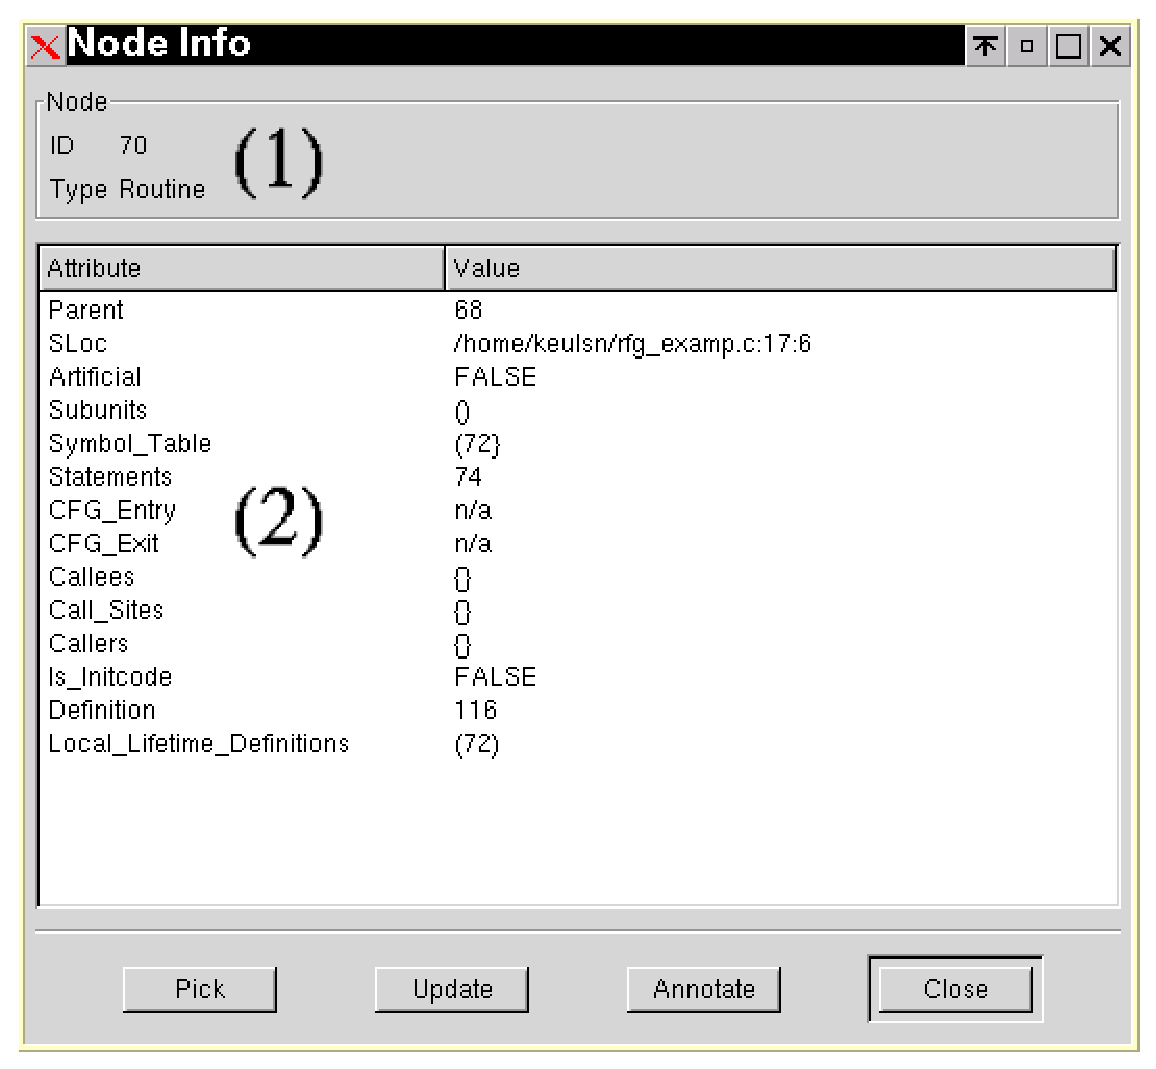
\includegraphics[scale=0.6]{gui/node_information_dialog}
       \caption{Node-Info-Window}
       \label{Node-Info-Window-Pic}
    \end{figure}

    In Knoten-Informationsfenstern (siehe Abbildung 
    \ref{Node-Info-Window-Pic}) 
    k�nnen n�here Informationen zu Fenster-Knoten angezeigt werden.\\
    
    Im Knoten-Informationsfenster wird die ID und die Knotenklasse des 
    vom Fenster-Knoten repr�sentierten IML-Knotens dargestellt (1),
    darunter befindet sich die Liste \gq{Attributes} mit den Attributen
    des Knotens (2).\\
    
    Unter der Liste (2) befinden sich nebeneinander die Buttons
    \gq{Pick}, \gq{Update}, \gq{Annotate} und \gq{Close}. 
    \gq{Pick} dient zur Auswahl eines anderen Fenster-Knotens 
    mittels des Fadenkreuzcursors, dazu wird nach Klicken von \gq{Pick}
    ein Fensterknoten angeklickt.\\
    
    \gq{Update} dient zur Aktualisierung der Liste, Annotate �ffnet das
    Knoten-Annotationsfenster (siehe Abschnitt \ref{Knoten Annotations-Dialog}).\\
    
    Die Informationen zu dem ausgew�hlten
    Fenster-Knoten werden dann im Knoten-Informationsfenster dargestellt.\\
    
    Das Knoten-Informationsfenster enth�lt, neben der Anzeige von Knoten-ID
    und Knoten-Typ, die Liste \gq{Attributes}:

    Die Liste Attributes enth�lt die Attribute des Knotens und hat
    zwei Spalten:
    
      \begin{enumerate}
        \item Name  (der Name des Attributes)
        \item Value (der Attributwert)
      \end{enumerate}
    

\clearpage
\section{Skriptdialog} \label{GUI Anfragedialog}

    \begin{figure}[!htbp]
       \centering
       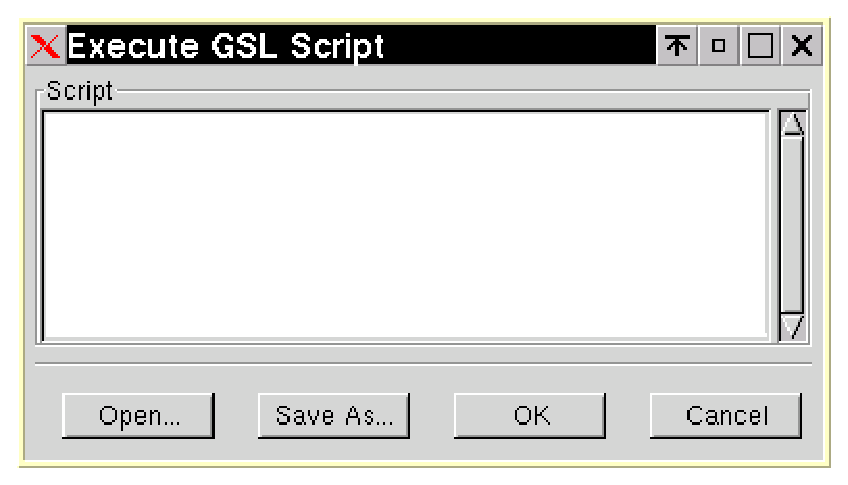
\includegraphics[scale=0.75]{gui/query_dialog}
       \caption{Skript-Dialog}
       \label{Skript-Dialog-Pic} 
    \end{figure}

Der Skriptdialog (siehe Abbildung \ref{Skript-Dialog-Pic})
hat zuoberst ein Textfeld,
in das ein GSL Skript eingegeben werden kann.

Unter Query Text befinden sich folgende Buttons:

      \begin{enumerate}
        \item Open...\\
           Mit diesem Button kann ein auf Festplatte gespeichertes Skript geladen werden.
           Nach Klick auf diesen Button erscheint ein Dateiauswahlfenster, nach Auswahl
           eines Skriptes wird dieses in das Textfeld eingef�gt.
        \item Save As...\\
           Mit diesem Button kann das im Textfeld eingetippte Skript gespeichert werden.
           Nach dem Klick auf diesen Button erscheint ein Dateiauswahlfenster, nach
           Festlegen eines Dateinamens wird das Skript unter diesem Namen gespeichert.
        \item Okay\\
           F�hrt das eingegebene Skript aus.
        \item Cancel
           Schlie�t das Fenster ohne Ausf�hrung oder Speicherung des Skriptes.
      \end{enumerate}
      
\clearpage
\section{Allgemeiner Texteingabedialog}
\label{DIALOG-WINDOW}

    \begin{figure}[!htbp]
       \centering
       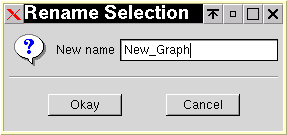
\includegraphics{gui/input_dialog}
       \caption{Dialog-Window}
       \label{Dialog-Window-Pic}
    \end{figure}

Ein allgemeiner Texteingabedialog ist ein Fenster Dialog Window 
(siehe Abbildung \ref{Dialog-Window-Pic}) mit dem
Titel \gq{Input}. Im Fenster ist ein einzeiliges Textfeld
mit einem Prompt-Text, zwei Buttons mit den Beschriftungen \gq{OK}
und \gq{Cancel}.

%\clearpage
\section{Set-Operation-Dialog}
\label{Common-Set-Operation-Dialog}

    \begin{figure}[!htbp]
       \centering
       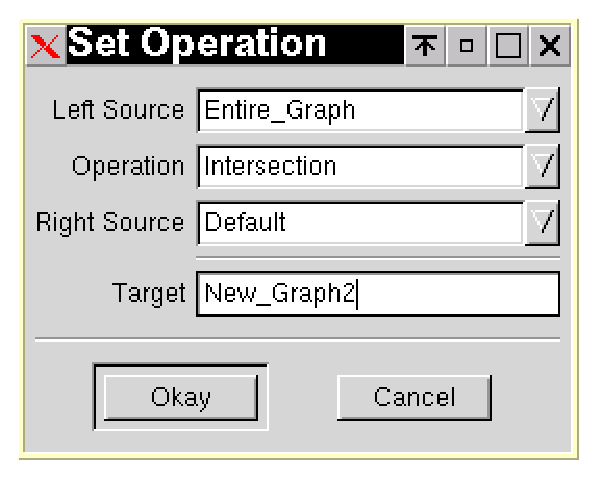
\includegraphics[scale=0.85]{gui/set_operation_dialog}
       \caption{Set-Operation-Dialog}
       \label{Set-Operation-Dialog-Pic}
    \end{figure}


Der Set-Operation-Dialog (siehe Abbildung \ref{Set-Operation-Dialog-Pic}) 
dient dazu, Mengenoperationen �ber 
Selektionen und
IML-Teilgraphen durchzuf�hren.
Die Mengenoperation l�sst sich wie folgt beschreiben:\\
TARGET := LEFT\_SOURCE <Operation> RIGHT\_SOURCE \\


Bestandteile des Dialoges sind:
\begin {enumerate}

 \item Left Source Combobox\\
 Soll eine Mengenoperation f�r Selektionen ausgef�hrt werden, so kann hier eine der
 Selektionen des entsprechenden Anzeigefensters ausgew�hlt werden.\\
 Bei einer Mengenoperation �ber IML-Teilgraphen, werden alle IML-Teilgraphen
 des Projektes angezeigt, von denen dann einer ausgew�hlt werden kann.
 
 \item Operation Combobox\\
 Mengenoperation, die ausgef�hrt werden soll; ausw�hlbar sind: Union, Difference oder Intersection.

 \item Right Source Combobox\\
 Soll eine Mengenoperation f�r Selektionen ausgef�hrt werden, so kann hier eine der
 Selektionen des entsprechenden Anzeigefensters ausgew�hlt werden.\\
 Bei einer Mengenoperation �ber IML-Teilgraphen, werden alle IML-Teilgraphen
 des Projektes angezeigt, von denen dann einer ausgew�hlt werden kann..
 
 \item Target Textfeld\\
 Name der neuen Selektion oder des neuen IML-Teilgraphen als Ergebnis
 der Mengenoperation.
 
 \item Buttons OK und Cancel\\
 Mit den beiden Buttons OK und Cancel l�sst sich die Operation starten bzw.
 der Dialog ohne Ausf�hren der Operation verlassen.
 
\end {enumerate}

 \clearpage
\section {Layoutalgorithmen Dialog}\label{Layoutalgorithmen-Dialog}

    \begin{figure}[!htbp]
       \centering
       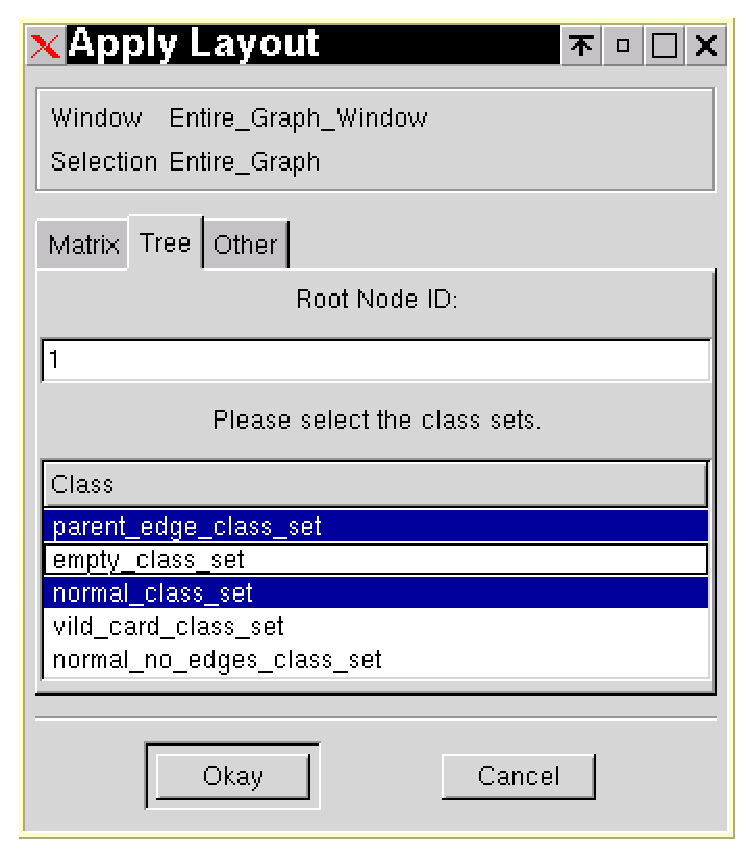
\includegraphics{gui/apply_layout_dialog}
       \caption{Layout-Algorithmen-Dialog}
       \label{Layout-Algorithm-Dialog-Pic}
    \end{figure}

Der Layoutalgorithmen Dialog (siehe Abbildung \ref{Layout-Algorithm-Dialog-Pic}) 
wird �ber Popup-Men�s auf Selektionen aufgerufen und bietet folgende M�glichkeiten:

\begin {enumerate} 
 \item Anzeige der zu layoutenden Selektion mit dem zu layoutenden Fenster (1)
 \item {Auswahl des Layoutalgorithmus}\\
       �ber die Tabs (4) im Fenster kann der Layoutalgorithmus ausgew�hlt werden,
       in der aktuellen Version stehen zur Auswahl: Matrix, Tree Layout,
       Other (f�r sp�tere Erweiterungen).\\
       Das Tree-Layout ordnet die Knoten als Baum an, dessen Wurzel anhand
       der ID des Knotens (welche u.a. mit dem Knoten-Informationsfenster, siehe
        \ref{Knoten-Informationsfenster}, festgestellt
       werden kann) festgelegt wird.\\
       Das Matrix-Layout ordnet die Knoten in einer Matrix an.\\
       
 \item Ggf.\ Eingabefeld f�r die ID des Wurzelknotens bei Treelayouts (2)
 \item {Ggf.\ Auswahl der f�r das Layout der Knoten zu ber�cksichtigenden Klassenmengen (3)
        (class sets, siehe \ref{Config-Klassenmengen} und \ref{Klassenmenge}) bei semantischen Tree-Layouts.}\\
        Nur Klassenmengen, die in der Liste per Mausklick markiert worden sind
        (Mehrfachmarkierungen sind m�glich), werden f�r das Layout
        ber�cksichtigt. Falls keine Klassenmengen angeben wurden,
        werden alle Kanten, {\em auch diejenigen, die nicht im Fenster
        sichtbar sind,} f�r das Layout verwendet.
 \item OK Button
 \item Cancel Button
\end {enumerate}

Nach dem Klicken von OK ist mit der linken Maustaste in ein Fenster auf den
dargestellten Anzeigeinhalt zu klicken (an einer leere Stelle), an dieser
Position wird dann die neu layoutete Selektion eingef�gt.

\clearpage
\section{Dateneingabe}
Beschreibung von verschiedenen GUI Elementen zur Eingabe von Daten.

\subsection{Knoten-Annotations-Dialog}
\label{Knoten Annotations-Dialog}

    \begin{figure}[!htbp]
       \centering
       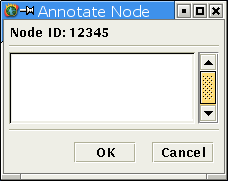
\includegraphics{gui/annotate_node}
       \caption{Node-Annotation-Dialog}
       \label{Node-Annotation-Dialog-Pic}
    \end{figure}
  
Der Knoten-Annotations-Dialog (siehe Abbildung 
\ref{Node-Annotation-Dialog-Pic}) besteht aus einem Fenster mit einem
Label, welches die ID des Knotens anzeigt, und einem Textfeld f�r den Annotationstext.
Mittels der beiden Buttons Okay und Cancel k�nnen die �nderungen im
Textfeld �bernommen oder verworfen werden. Der Button Delete kann dazu
verwendet werden, das Textfeld zu leeren.
\index{Knoten-Annotationen}


%  \clearpage
\subsection{Platz Schaffen-Dialog}
\label{Platz Schaffen-Dialog}

    \begin{figure}[!htbp]
       \centering
       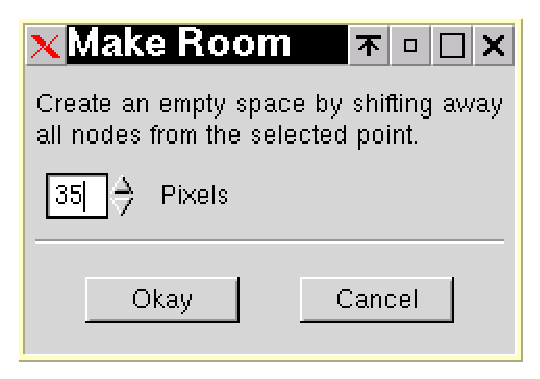
\includegraphics{gui/make_room}
       \caption{Make-Room-Dialog}
       \label{Make-Room-Dialog-Pic}
    \end{figure}

Im Dialogfenster Make Room (siehe Abbildung \ref{Make-Room-Dialog-Pic}) 
wird in einem Textfeld als Zahl 
eingegeben, um wie viel
Pixel die Fenster-Knoten an einer vorher markierten Stelle auseinandergeschoben 
werden sollen.
Mit dem Button Okay kann best�tigt werden, mit dem Button Cancel abgebrochen werden.

\clearpage
\section{Ausgabe von Fehlermeldungen}
\label {GUI Ausgabe von Fehlermeldungen}

    \begin{figure}[!htbp]
       \centering
       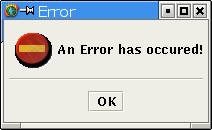
\includegraphics{gui/error_dialog}
       \caption{Error-Window}
       \label{Error-Window-Pic}
    \end{figure}

Im Fenster eines allgemeinen Fehlerdialoges (siehe Abbildung \ref{Error-Window-Pic})
befindet sich die Fehlermeldung und ein \gq{OK}-Button, mit dem das
Fenster geschlossen werden kann.. 

\section{Sicherheitsabfrage}\label{Sicherheitsabfrage}
\index{Sicherheitsabfrage}

    \begin{figure}[!htbp]
       \centering
       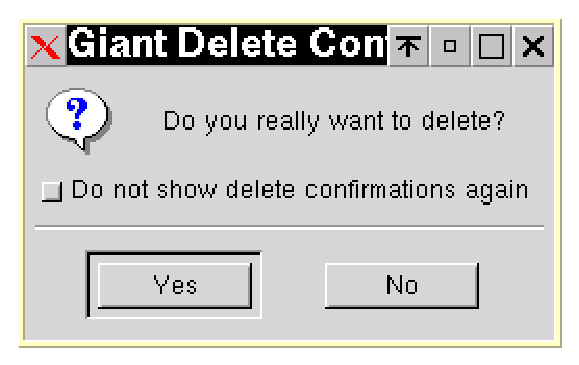
\includegraphics{gui/confirmation_dialog}
       \caption{Confirmation-Window}
       \label{Confirmation-Window-Pic}
    \end{figure}
    
Eine allgemeine Sicherheitsabfrage (siehe Abbildung \ref{Confirmation-Window-Pic}) 
besitzt einen
Fragetext und die zwei Buttons \gq{Yes} und \gq{No}.
Ggf. kann mit einem Radiobutton festgelegt werden, da� Sicherheitsabfragen
des jeweiligen Types in Zukunft nicht mehr angezeigt werden (z.B. \gq{Do not
show delete confirmations again}).

\clearpage

\section{Auswahl von Dateien}

  \subsection {Der \gq{Standard-Filechooser-Dialog}}
  \label {Standard-Filechooser-Dialog}

    \begin{figure}[!htbp]
       \centering
       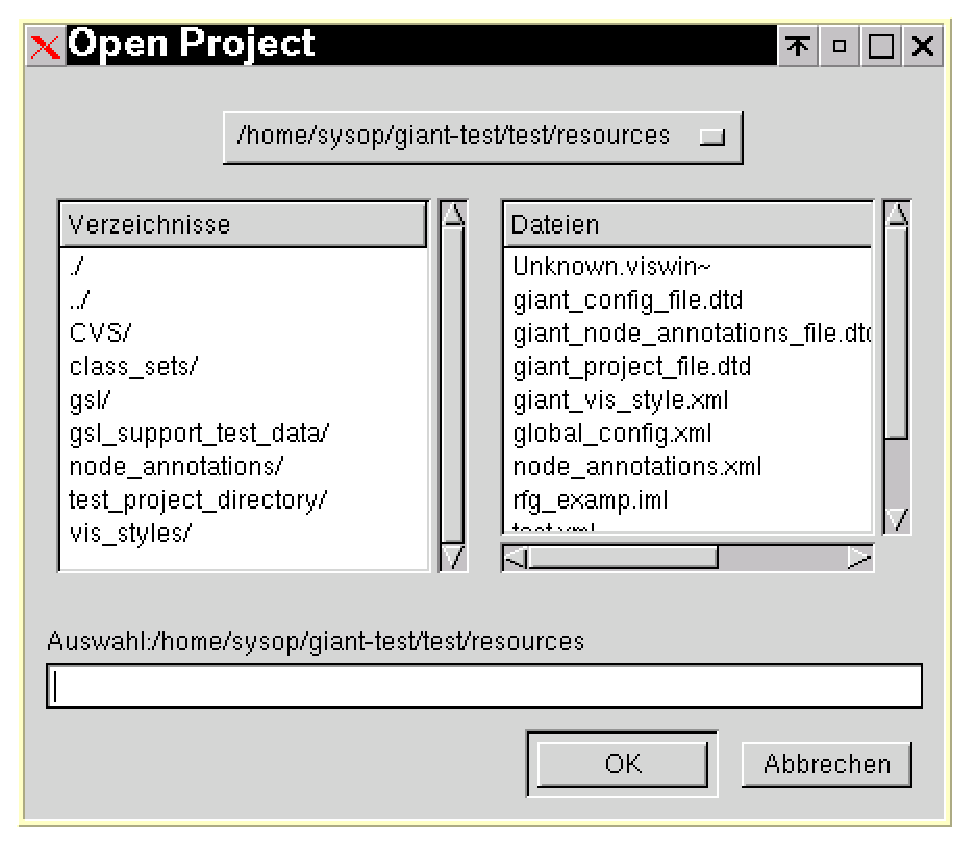
\includegraphics{gui/filechooser_dialog}
       \caption{Filechooser-Window}
       \label{Filechooser-Window-Pic}
    \end{figure}

Die Auswahl von Dateien (Laden/Speichern) passiert bei GIANT mittels
des Standard-Filechooser-Dialogs (siehe Abbildung \ref{Filechooser-Window-Pic}). 
Dieser Dialog ist Bestandteil der Widget-Bibliothek von GTK.


% ******** Gibt es den Fadenkreuz-Cursor?
\section{Fadenkreuz-Cursor}
\label{Fadenkreuzcursor}
        Der Cursor verwandelt sich nach Auswahl bestimmter
        Funktionen (siehe z.B. Funktion \ref{Platz Schaffen-Dialog}) in ein Fadenkreuz.
        Durch Linksklick auf einen Fenster-Knoten oder eine 
        Fenster-Kante in einem Anzeigefenster  
        wird diese(r) f�r die jeweilige Funktion ausgew�hlt. 
        Der Fadenkreuz-Cursor wird auch zur Vorgabe von Positionen,
        an denen dann z.B. neue Fenster-Knoten eingef�gt werden,
        verwendet.
        Nach dem Linksklick  verwandelt
        sich der Fadenkreuz-Cursor wieder in den Standard-Cursor.
        Durch einen Rechtsklick bei aktivem Fadenkreuz-Cursor l�sst sich 
        die aktuelle Funktion abbrechen.




%%% Local Variables: 
%%% TeX-master: "spec"
%%% End: 



%===============================================================================
% 
% Anfragesprache
%
\chapter{GIANT Scripting Language}
\label {GIANT Scripting Language}

Die F�higkeiten der GIANT Scripting Language (GSL) werden im Anhang 
\gq{GSL}, der Teil der GIANT Spezifikation ist, beschrieben.

\section{GSL-FAQ}
\subsection{Wie starte ich GSL?}
Zwei M�glichkeiten:

\begin{itemize}
  \item �ber Kommandozeile
  \item �ber Query-Dialog
\end{itemize}

Dar�berhinaus gibt es noch die M�glichkeit, vorgefertige Skripte �ber
die Men�s zu starten. 

\subsection{Mein Script bei if funktioniert nicht als condition}
So ist das auch nicht spezifiziert. Abhilfe:

\begin{verbatim}
  // ...
  +start_cond;
  if
    (is_script (b),
     {() set ('start_cond, b ())},
     {() set ('start_cond, b   )});
  if
    (start_cond,
    // ...
\end{verbatim}

Wichtig ist hier, dass beide Zweige als Skripte implementiert
sind. Siehe auch Frage \ref{if_eval}.

\subsection{If f�hrt immer beide Zweige aus}
\label{if_eval}
Beispiel:

\begin{verbatim}
  if 
    (true,
     set ('a, 10),
     set ('a, 20))
\end{verbatim}

a ist jetzt 20 und nicht 10.

Der Grund liegt in der Auswertung: if ist auch ein GSL-Skript. Um ein
Skript auszuf�hren, werden zuerst die Parameter f�r dieses Skript
interpretiert und das Ergebnis dieser Interpretation dem Skript
�bergeben. Bei obigem Beispiel sind das true, 10 und 20, da die
Skripte \verb1set ('a, 10)1 und \verb1set ('a, 20)1 \gq{ausgef�hrt}
wurden. Nachdem true true ist, wird 10 ausgewertet, was zu 10 f�hrt.

Richtig ist deshalb:

\begin{verbatim}
  if 
    (true,
     {() set ('a, 10)},
     {() set ('a, 20)})
\end{verbatim}

Hier in den Zweigen nach der Auswertung und vor der \gq{Ausf�hrung}
von if Aktivierungsinformationen liegen. Und so wird nach der
Entscheidung, welcher Zweig ausgewertet werden soll, die
Aktivierungsinformationen zu Skripten ausgewertet.

%===============================================================================
% 
% Projektverwaltung
%
\chapter{GIANT Projektverwaltung}
\label{GIANT Projektverwaltung}

In diesem Kapitel wird beschrieben, wie persistente Arbeitsergebnisse
von GIANT strukturiert und gespeichert werden.
Arbeitsergebnisse sind z.B. vom Benutzer erzeugte Anzeigefenster
mit als Fenster-Knoten visualisierten IML-Knoten eines IML-Graphen.
Soweit f�r das Verst�ndnis von GIANT n�tig, sind auch Interna des
Programms festgehalten.

% ==============================================================================
%  $RCSfile: project.tex,v $, $Revision: 1.17 $
%  $Date: 2003/02/25 14:33:49 $
%  $Author: squig $
%
%  Description:
%
% ==============================================================================


%===================
\section {Persistenz �ber Projekte}

GIANT speichert persistente Informationen in so genannten Projekten.
\begin {enumerate}

  \item 
  Wird w�hrend des Betriebs von GIANT ein neues Projekt angelegt, so erh�lt 
  es automatisch eine Projektdatei.
  
  \item
  Ein Projekt besteht aus einem Verweis auf eine IML-Graph-Datei, auf die sich
  die gespeicherten Informationen beziehen, sowie aus den gespeicherten 
  Informationen f�r IML-Teilgraphen, Anzeigefenster und Knoten-Annotationen.
 
  \item
  Jedes Projekt hat einen vom Benutzer definierbaren Namen, dieser Name 
  entspricht dem Namen der Projektdatei und wird innerhalb des IML-Browsers 
  angezeigt.

  \item
  Der Name eines bereits angelegten Projektes kann mit den Mitteln von 
  GIANT nicht ge�ndert werden (au�er dadurch, dass  man das Projekt unter 
  neuem Namen neu speichert). 

  \item
  Der Benutzer kann beliebig viele Projekte anlegen.
  
  \item
  In GIANT darf immer nur ein Projekt gleichzeitig ge�ffnet sein. 
  
  \item
  W�hrend der Arbeit mit GIANT kann jederzeit ein Projekt geladen oder ein
  neues Projekt angelegt werden. 
  Voraussetzung hierf�r ist allerdings, dass dies 
  in der Reflektion zum IML-Graphen unterst�tzt wird.
  
  \item
  GIANT wei� nicht, ob ein geladenes Projekt gegen�ber den f�r das Projekt
  in der Projektdatei und in den Verwaltungssdateien gespeicherten 
  Informationen modifiziert wurde oder nicht.

\end {enumerate}


  \subsection {Das Projektverzeichnis}
  \begin {enumerate}

    \item  
    S�mtliche Dateien, die die Informationen f�r ein Projekt enthalten,
    befinden sich in diesem Verzeichnis. 

    \item
    In einem Projektverzeichnis darf nur ein Projekt abgelegt werden.
    
  \end {enumerate}    


  \subsection {Die Projektdatei}
  \begin {enumerate}

    \item
    Die Projektdatei liegt als XML-Datei vor.

    \item
    Die Projektdatei befindet sich im Projektverzeichnis und enth�lt 
    Informationen, die zur Identifikation des zu einem Projekt geh�renden 
    IML-Graphen n�tig sind. 
  
    \item
    Der Name der Projektdatei entspricht dem Namen des Projektes.

    \item
    Die Projektdatei enth�lt Referenzen zu allen Dateien, die Bestandteil
    des Projektes sind (Verwaltungsdateien f�r IML-Teilgraphen und
    Anzeigefenster und die Verwaltungsdatei f�r Knoten-Annotationen).

    \item
    Der Pfad zu der Datei, die den IML-Graphen enth�lt, ist in der Projektdatei 
    gespeichert. 
  \end {enumerate}
  
 
  \subsection {Pr�fung der IML-Graph Datei}
  Die Reflektion muss f�r jede IML-Graph Datei eine m�glichst eindeutige 
  Pr�fsumme berechnen k�nnen. Beim Laden eines Projektes wird �berpr�ft, 
  ob die in der Projektdatei gespeicherte Pr�fsumme
  der Pr�fsumme der zu ladenden IML-Graph Datei entspricht. 
  Das Verhalten von GIANT f�r den Fall, dass eine IML-Graph Datei geladen wird, 
  die zwar die passende Pr�fsumme hat, aber nicht den IML-Graphen enth�lt, 
  der dem Projekt eigentlich zu Grunde liegt, ist undefiniert.


  \subsection {Verwaltungsdateien f�r Anzeigefenster}
 
  \begin {enumerate}
  
    \item
    Zu jedem Anzeigefenster gibt es eine Verwaltungsdatei. 
    
    \item
    Diese Verwaltungsdatei enth�lt alle Informationen zur kompletten 
    Rekonstruktion eines Anzeigefensters. Alle Informationen werden
    in bin�rer Form gespeichert.
 
  \end {enumerate}
  Insbesondere werden folgende Informationen gespeichert:
 
  \begin {enumerate}
 
    \item Der komplette Anzeigeinhalt 
          (alle visualisierten Knoten und Kanten mit Position).
    \item Alle Pins (gespeicherte sichtbare Anzeigeinhalte).
    \item Alle dem Anzeigefenster bekannten Selektionen.
 
  \end {enumerate}
 
  Der f�r das Anzeigefenster gew�hlte Visualisierungsstiel wird zwar mit 
  gespeichert, da die Viualisierungsstiele v�llig unabh�ngig von den 
  Projekten �ber Konfigurationsdateien realisiert werden, 
  kann nicht gerantiert werden, dass der gew�nschte Stiel beim Laden 
  des Projektes auch wieder gefunden wird,
  in diesem Fall wird dann ein \gq{Standard-Stil} verwendet.


  \subsection {Verwaltungsdateien f�r IML-Teilgraphen}
  \begin {enumerate}

   \item
    F�r jeden IML-Teilgraphen gibt es eine eigene Verwaltungsdatei.
    
    \item
    S�mtliche erzeugten IML-Teilgraphen werden in Verwaltungsdateien in 
    bin�rer Form gespeichert. 

  \end{enumerate}
  
  
  \subsection {Die Verwaltungsdatei f�r Knoten-Annotationen}
  \begin {enumerate}

   \item
   Alle Knoten-Annotationen werden in einer Verwaltungsdatei gespeichert.
   
   \item
   Diese Datei liegt als XML Datei vor.
  \end{enumerate}
  

 
 
%===================
\section {Grundlegendes Verhalten von GIANT beim Speichern von Projekten} 
  

  \subsection{\gq{Alles Speichern}}\label{Alles Speichern}
  Diese Funktionalit�t wird von entsprechenden UseCases genutzt. 
  Hierbei werden alle Anzeigefenster, IML-Teilgraphen 
  und Knoten-Annotationen in die Verwaltungsdateien geschrieben, 
  wobei alle �nderungen an noch offenen Anzeigefenstern ber�cksichtigt 
  werden.\\
 

  %===
  \subsection {Persistenz von Anzeigefenstern}
  \begin {enumerate}

    \item
    S�mtliche dem Projekt bekannten Anzeigefenster (alle Anzeigefenster zu 
    denen es eine entsprechende Verwaltungsdatei gibt) werden auf der GUI in 
    der Liste �ber die Anzeigefenster angezeigt, egal ob sie ge�ffnet sind
    oder nicht. 

    \item 
    Zu jedem Anzeigefenster eines Projektes gibt es eine Verwaltungsdatei,
    beim �ffnen eines neuen Fensters wird diese Datei automatisch mit
    erzeugt.

    \item
    Wird ein ge�ffnetes Anzeigefenster geschlossen, 
    so fragt GIANT nach, ob es eventuelle �nderungen speichern soll
    oder nicht. Falls ja, werden eventuelle �nderungen in die f�r das 
    Anzeigefenster vorhandene Verwaltungsdatei geschrieben, 
    anderenfalls bleibt der Zustand des Anzeigefensters nach der letzten
    Speicherung vorhanden (die zugeh�rige Verwaltungsdatei wird nicht 
    ver�ndert).

    \item
    Modifikationen (z.B. das Verschieben von Knoten) 
    auf einem Anzeigefenster werden nicht automatisch
    nach deren Durchf�hrung gespeichert (so kann notfalls ein
    Undo durchgef�hrt werden).

    \item
    Ein zu einem Projekt geh�rendes Anzeigefenster kann gel�scht werden, 
    hierbei werden alle Information �ber das Anzeigefenster einschlie�lich
    der Verwaltungsdatei vernichtet.
    >>>>>>>>>>>>>>>>USE CASE - L�schen persistenter Anzeigefenster
  \end {enumerate}

  %===
  \subsection {Persistenz von IML-Teilgraphen}
  \begin {enumerate}

    \item
    Alle in einem Projekt bereits vorhandenen IML-Teilgraphen werden auf der 
    GUI angezeigt (in einer entsprechenden Liste).
  
    \item
    Neu erzeugte IML-Teilgraphen und �nderungen an bestehenden 
    IML-Teilgraphen k�nnen �ber \gq{alles Speichern} (siehe oben) 
    gespeichert werden.
       
    \item
    Wird das Programm beendet, ohne das zuvor \gq{Alles Speichern} ausgef�hrt 
    worden ist, so gehen  alle nicht gespeicherten Informationen zu den 
    IML-Teilgraphen verloren (alle zwischenzeitlich ausgef�hrten Modifikationen 
    und alle zwischenzeitlich neu erzeugten IML-Teilgraphen). 
    Der Zustand des Projektes  nach dem letzten Speichern bleibt dann erhalten.

    \item
    Modifikationen an bestehenden IML-Teilgraphen werden nicht automatisch 
    gespeichert, zu neu erzeugten IML-Teilgraphen wird nicht automatisch
    eine Verwaltungsdatei erzeugt.
    \\
    N�TIG; DA SONST ANFRAGEN EVENTUELL AUSGEBREMST.
    IM GEGENSATZ ZU ANZEIGEFENSTERN KANN MAN IML-TEILGRAPHEN NICHT �FFNEN
    IM GEGENSATZ ZU ANZEIGEFENSTERN (fliegen beim Schlie�en aus dem
    speicher raus) WERDEN ALL IML-TEILGRAPHEN pauschal im
    SPEICHER GEHALTEN.

    \item
    IML-Teilgraphen k�nnen gel�scht werden. Falls vorhanden, wird dann auch
    die entsprechende Verwaltungsdatei ebenfalls sofort gel�scht.
  \end {enumerate}
  
  
  
\subsection {Persistenz von Knoten-Annotationen}
  \begin {enumerate}
  
   \item
   �nderungen bestehender oder neu erzeugte Knoten-Annotationen werden nur
   �ber die Funktionali�t unter \gq{alles Speichern} in die 
   Verwaltungsdatei geschrieben.
   
   \item
   Einmal erzeugte Knoten-Annotationen werden jedem IML-Knoten mit der 
   entsprechenden ID zugeordnet, egal in welchem Anzeigefenster diese
   visualisiert sind. Ein Knoten kann auch annotiert sein, wenn er in keinem
   Anzeigefenster visualisiert ist. Wird ein annotierter Knoten gel�scht 
   (aus einem Anzeigefenster entfernt), so wird der dazu vorhandene 
   Eintrag f�r die Annotation in der Verwaltungsdatei nicht automatisch mit gel�scht.
   
   >>>>>>>>>>>>>>>> EVENTUELL M�SSEN WIR HIER EINEN FILTER BAUEN
   DER KNOTEN-Annotationen entfernt, die nicht mehr gebraucht werden.
   
 \end {enumerate}
  
  
  
  
  
  
  
  
  


%===============================================================================
% 
% Beschreibung aller Konfigurationsdateien
%
\chapter{Konfiguration von GIANT}
\label{Konfiguration von GIANT}

Hier wird beschrieben, wie benutzerdefinierbare Einstellungen von
GIANT gespeichert und verwaltet werden. In diesem Kapitel wird 
insbesondere beschrieben, welche Einstellungen der Benutzer
in welchen Konfigurationsdateien vornehmen kann.

% ==============================================================================
%  $RCSfile: config.tex,v $, $Revision: 1.35 $
%  $Date: 2003/04/21 01:13:30 $
%  $Author: schwiemn $
%
%  Description:
%
%  Last-Ispelled-Revision: 1.19
%
% ==============================================================================


\section {Allgemeines} \index{Konfiguration}
\begin {enumerate}

  \item
  S�mtliche konfigurierbaren Einstellungen werden in XML-Dateien vorgenommen.
  F�r die verschiedenen Dateitypen werden auch
  Dokumenttyp-Definitionen (DTDs) erstellt.
  
  \item \label{config-allgemeines-punkt2}
  \index{Konfigurationsdatei!globale}
  Es gibt genau eine \gq{globale Konfigurationsdatei}. Zudem kann es beliebig 
  viele weitere XML-Dateien zur Konfiguration der weiter unten beschriebenen 
  Visualisierungsstile geben.\\
  Diese Dateien liegen in einem von GIANT fest vorgegebenen Verzeichnis.
  
  \item \index{Konfigurationsdatei!benutzerdefinierte}
  Die unter Punkt \ref{config-allgemeines-punkt2} beschriebenen Dateien zu
  Konfiguration k�nnen vom Benutzer auch in einem separaten 
  Unterverzeichnis seines Home-Verzeichnisses abgelegt werden. Findet
  GIANT beim Start ein derartiges Verzeichnis, so werden die
  Einstellungen aus der dort vorgefundenen Konfigurationsdatei, sowie
  die dort vorgefundenen Visualisierungsstile geladen.
 
\end {enumerate}


\section {Die globale Konfigurationsdatei} \index{Konfigurationsdatei}
Diese Datei ist in XML verfasst. In Ihr k�nnen die anschlie�end beschriebenen
Einstellungen vorgenommen werden.

%EVENTUELL F�R JEDEN BENUTZER EIGENE KONFIGURATIONS-DATEI VORSEHEN.

  \subsection {Verweise auf GSL-Skripte} 
  \index{Makros}
  \index{GSL!Makros}
  Es k�nnen GSL-Skript-Makros definiert werden. Jeder Makro wird durch 
  einen eindeutigen Namen und durch einen Verweis
  auf die Datei, welche das GSL-Skript enth�lt, spezifiziert.
  Der Makro kann dann aus einem Popup-Men� heraus aufgerufen werden, wobei
  dann das in der Datei stehende GSL Skript ausgef�hrt wird.

  \subsection {Farbe von Hervorhebungen}
  \index{hervorheben!Farben konfigurieren}
  Einstellung der Farben, mittels derer Selektionen oder IML-Teilgraphen 
  hervorgehoben werden.
  \begin {enumerate}
    \item Eine beliebige Farbe f�r die aktuelle Selektion.
    \item Beliebige Farben f�r das
          Hervorheben weiterer Selektionen.
    \item Beliebige Farben f�r das 
          Hervorheben von IML-Teilgraphen.
  \end {enumerate}

  \subsection {Editor zur Anzeige des Quellcodes}
  \label{Konfig Editor zur Anzeige des Quellcodes}
  \index{Editoren!Anzeige des Quellcodes}

  Der Benutzer legt in der globalen Konfigurationsdatei fest, 
  mit welchem Editor der zu IML-Knoten korrespondierende
  Quellcode automatisch angezeigt wird (unterst�tzt werden Emacs und vi). 

\section {Visualisierungsstile} \label{Config Visualisierungsstile}
\index{Visualisierungsstile!Konfiguration}
\index{Konfiguration!Visualisierungsstile}

Der Benutzer kann beliebig viele Visualisierungsstile definieren.
Mittels dieser Visualisierungsstile kann die Darstellung von
Fenster-Knoten und Fenster-Kanten dynamisch zur Laufzeit ge�ndert werden
(siehe auch 
\ref{Den Visualisierungsstil eines Anzeigefensters �ndern}).
Weitere Informationen zur Visualisierung von Fenster-Knoten und
Fenster-Kanten sind unter den Abschnitten
\ref{Visualization Visualisierung von Kanten} und
\ref{Visualization Visualisierung von Knoten} zu finden.\\
F�r die Visualisierungsstile gelten die folgenden Konventionen:


\begin {enumerate}

  \item
  F�r jeden Visualisierungsstil muss es eine entsprechende XML-Datei geben. 

  \item
  Ein Visualisierungsstil beschreibt, wie die Knoten und Kanten des 
  IML-Graphen innerhalb eines Anzeigefensters graphisch dargestellt 
  werden k�nnen.

  \item
  In einem Visualisierungsstil k�nnen klassenspezifische Einstellungen 
  vorgenommen werden, die nur f�r Knoten und Kanten gelten, 
  die zu der entsprechenden Klasse geh�ren.
  Bei jeder klassenspezifischen Einstellung f�r Knoten und Kanten kann daher 
  eine Liste der betroffenen Knoten- und Kantenklassen angegeben werden, 
  f�r die diese Einstellungen gelten sollen.

  \item
  Wird eine Kanten- oder eine Knotenklasse innerhalb eines
  Visualisierungsstils mehreren klassenspezifischen Einstellungen zugeordnet,   
  f�hrt dies zu keinem Fehler, es bleibt aber unspezifiziert, 
  welche Einstellung tats�chlich genommen wird.

  \item
  Es gibt jeweils eine Standard-Einstellung, die f�r alle
  Knoten- und Kantenklassen genommen wird, f�r die keine
  extra klassenspezifischen Einstellungen vorgenommen wurden.

  \item \index{Visualisierungsstile!Standard-Visualisierungsstil}
  Es gibt immer einen von GIANT fest
  vorgegeben Standard-Visualisierungsstil. Dieser Visualisierungsstil
  wird f�r neu erzeugte Anzeigefenster genommen. 
  Kann GIANT den einem Anzeigefenster zugewiesenen Visualisierungsstil
  nicht finden (falls die zugeh�rige XML-Datei fehlt) wird ebenfalls
  der Standard-Visualisierungsstil genommen. 

\end {enumerate}


  \subsection {Name des Visualisierungsstils}
  Jeder Visualisierungsstil erh�lt einen Namen. Unter diesem Namen ist der 
  Visualisierungsstil f�r jedes Anzeigefenster einzeln ausw�hlbar.
 
  \subsection {Einstellungen innerhalb des Visualisierungsstils}
    \begin{enumerate}
      \item Die Hintergrundfarbe im Anzeigefenster.

     % \item Wann Kanten im sichtbaren Anzeigeinhalt angezeigt werden sollen.
 
     %  \subitem Nur falls Start- und Zielknoten ebenfalls im sichtbaren 
     %           Anzeigeinhalt.
     %  \subitem Auch anzeigen falls nur Startknoten im sichtbaren 
     %           Anzeigeinhalt.
     %  \subitem Auch anzeigen falls nur Zielknoten im sichtbaren Anzeigeinhalt.
     %  \subitem Auch anzeigen falls weder Start- und Zielknoten im sichtbaren 
     %           Anzeigeinhalt. 
    \end{enumerate}


  \subsection {Klassenspezifische Einstellungen f�r Knoten}
  \index{Visualisierungsstile!klassenspezifische Einstellungen}

  Folgende  Einstellungen k�nnen f�r Knotenklassen vorgenommen werden. 
  Es muss eine Standard-Einstellung erstellt werden, die f�r alle
  Knotenklassen angewendet wird, f�r die nichts anderes definiert ist.
  \begin{enumerate}  
  

    \item Ein Icon f�r die Knotenklasse (Verweis auf eine entsprechende 
          Bilddatei). Das Icon muss im Pixmap-Format 
          vorliegen. Die Gr��e des Icons ist beliebig, bei zu gro�en
          Icons wird abgeschnitten. Es wird garantiert, dass Icons
          bis zu einer Gr�\ss e von 32*32 Pixel komplett dargestellt werden
          k�nnen.

    \item Eine Liste der Attribute der Knotenklasse, welche direkt innerhalb 
          des Anzeigefensters in dem \gq{Rechteck} f�r den Knoten dargestellt 
          werden sollen.
    \item Die Farbe der Schrift, mit der die Informationen innerhalb
          des Knoten-Rechtecks dargestellt werden.
    \item Die F�llfarbe des \gq{Rechtecks} in welchem die Attribute zu dem 
          Knoten dargestellt werden.
    \item Die Rahmenfarbe des \gq{Rechtecks}.
    
  \end{enumerate}

  
  \subsection {Klassenspezifische Einstellungen f�r Kanten}
  Folgende Einstellungen k�nnen f�r Kantenklassen vorgenommen werden.
  Es muss eine Standard-Einstellung erstellt werden, die f�r alle
  Kantenklassen angewendet wird, f�r die nichts anderes definiert ist.
  \begin{enumerate}
    \item Die Farbe der Kante.
    \item Die Farbe der Kantenbeschriftung.
    \item Die Art der Linie der Kante (normal, gestrichelt).
    \item Ob die Kante mit ihrer Kantenklasse beschriftet werden soll oder 
          nicht.
  \end{enumerate}

  Eine Kantenklasse wird durch die Knotenklasse des Start-Knotens 
  und durch den Namen des Attributes, welches die Kante darstellt, 
  eindeutig festgelegt (siehe Begriffslexikon). 
  Will der Benutzer nun Einstellungen f�r
  Kantenklassen vornehmen, kann er sich entweder auf genau eine
  Kantenklasse \gq{Start-Knotenklasse.Attributname} beziehen oder
  mittels eines Platzhalters auch auf mehrere:

  \begin{enumerate}
    \item Der Benutzer kann mittels des Platzhalters \gq{*}
          eine klassenspezifische Einstellung f�r
          alle Kanten, deren Start-Knoten zu einer bestimmten
          Knotenklasse geh�rt, 
          vornehmen -- also \gq{Start-Knotenklasse.*}.

   \item  Der Benutzer kann mittels des Platzhalters \gq{*}
          eine klassenspezifische Einstellung f�r
          alle Kanten, bei denen das sie repr�sentierende Attribut
          den gleichen Namen hat,
          vornehmen -- also \gq{*.Attributname}.
 
  \end{enumerate}

  
\section {Skript-Dateien} 
\label {Config Anfrage-Dateien}
\index{GSL!Skriptdateien} \index{Skriptdateien}

Eine Skript-Datei ist eine Textdatei, die genau ein GSL Skript enth�lt.
Auf diese Art und Weise k�nnen komplexe Skripte gespeichert und 
wiederverwendet werden.\\
Geladen werden k�nnen solche Dateien beim Kommandozeilenaufruf 
(siehe \ref{fa Starten von GIANT})
oder im Dialog zur Eingabe eine Skripts 
(vgl.\ UseCase \ref{UC Anfrage laden}).
F�r eine exakte Spezifikation der GSL siehe Kapitel 
\ref {GIANT Scripting Language}. 



%==============================================================================
%
%  Index
%
\printindex

%==============================================================================
% 
% Anhang
%
\newpage
\appendix

\end{document}
